% =====================================================================
%  MATH 55 -- Lecture Notes & Reviewer No. 6
%  Directional Derivatives and the Gradient Vector
%  Build: latexmk -pdf -outdir=build lecture-notes-02.tex
% =====================================================================
\documentclass[11pt,a4paper]{article}

\newcommand{\NotesNumber}{6}
\newcommand{\NotesKind}{Lecture Notes \& Reviewer No.~6}
\newcommand{\NotesShortTitle}{Directional Derivatives}
\newcommand{\NotesPdfTitle}{MATH 55 Lecture Notes 6: Directional Derivatives and the Gradient Vector}
% =====================================================================
%  MATH 55 -- Shared preamble for the Second Long Exam reviewers
%  Reproduces the look of "Lecture Notes 01" (Lecture Notes & Reviewer
%  No. 5): Latin Modern, small-caps running heads, ruled chapter titles,
%  amsthm environments numbered within chapters, framed strategy boxes.
%
%  Each document defines, BEFORE \input-ing this file:
%     \NotesNumber      e.g. 6
%     \NotesKind        e.g. Lecture Notes \& Reviewer No.~6
%     \NotesShortTitle  e.g. Directional Derivatives and Gradient
%     \NotesPdfTitle    plain-text title for the PDF metadata
% =====================================================================

% ---------- Fonts and encoding --------------------------------------
\usepackage[T1]{fontenc}
\usepackage[utf8]{inputenc}
\usepackage{lmodern}
\usepackage{microtype}

% ---------- Page geometry -------------------------------------------
\usepackage[a4paper,top=1in,bottom=1in,left=1.05in,right=1.05in,
            headheight=15pt,footskip=30pt]{geometry}
\setlength{\parindent}{0pt}
\setlength{\parskip}{6pt plus 2pt minus 1pt}

% ---------- Mathematics ---------------------------------------------
\usepackage{amsmath,amssymb,amsthm,mathtools}
\usepackage{bm}

% ---------- Graphics, tables, lists ---------------------------------
\usepackage{graphicx}
\usepackage[dvipsnames]{xcolor}
\usepackage{tikz}
\usetikzlibrary{arrows.meta,calc,angles,quotes,positioning}
\usepackage{pgfplots}
\pgfplotsset{compat=1.17}
\usepackage{booktabs,array,tabularx,multirow}
\usepackage{caption}
\usepackage{subcaption}
\captionsetup{font=small,labelfont=bf,width=0.92\linewidth}
\usepackage{enumitem}
\setlist{itemsep=2pt,topsep=4pt}
\usepackage{float}
\usepackage[most]{tcolorbox}

% ---------- Headings --------------------------------------------------
\usepackage{titlesec}
% "Chapter N" over a ruled small-caps title, each on a new page
\titleformat{\section}[display]
  {\normalfont\centering}
  {\large\scshape Chapter \thesection}
  {8pt}
  {\titlerule\vspace{10pt}\LARGE\scshape}
  [\vspace{4pt}\titlerule]
\titlespacing*{\section}{0pt}{0pt}{22pt}
\newcommand{\sectionbreak}{\clearpage}
\titleformat{\subsection}{\normalfont\large\bfseries}{\thesubsection}{1em}{}
\titleformat{\subsubsection}{\normalfont\normalsize\bfseries}{\thesubsubsection}{1em}{}
\setcounter{tocdepth}{2}

% Appendices are titled "Appendix A" instead of "Chapter A"
\newcommand{\startappendix}{%
  \appendix
  \titleformat{\section}[display]
    {\normalfont\centering}
    {\large\scshape Appendix \thesection}
    {8pt}
    {\titlerule\vspace{10pt}\LARGE\scshape}
    [\vspace{4pt}\titlerule]%
}

% ---------- Running heads and feet ----------------------------------
\usepackage{fancyhdr}
\newcommand{\NotesAuthor}{Juevesano, D.}
\fancypagestyle{m55}{%
  \fancyhf{}%
  \fancyhead[L]{\small\textsc{\NotesKind}}%
  \fancyhead[R]{\small\textsc{Math 55 -- \NotesShortTitle}}%
  \fancyfoot[L]{\small\NotesAuthor\ 2026 ALL RIGHTS RESERVED. Not for redistribution.}%
  \fancyfoot[R]{\small\thepage}%
  \renewcommand{\headrulewidth}{0.4pt}%
  \renewcommand{\footrulewidth}{0.4pt}%
}
% chapter-opening pages use "plain": keep the same head/foot there too
\fancypagestyle{plain}{%
  \fancyhf{}%
  \fancyhead[L]{\small\textsc{\NotesKind}}%
  \fancyhead[R]{\small\textsc{Math 55 -- \NotesShortTitle}}%
  \fancyfoot[L]{\small\NotesAuthor\ 2026 ALL RIGHTS RESERVED. Not for redistribution.}%
  \fancyfoot[R]{\small\thepage}%
  \renewcommand{\headrulewidth}{0.4pt}%
  \renewcommand{\footrulewidth}{0.4pt}%
}
\pagestyle{m55}

% ---------- Theorem-like environments --------------------------------
\theoremstyle{definition}
\newtheorem{definition}{Definition}[section]
\newtheorem{example}[definition]{Example}
\newtheorem{problem}[definition]{Problem}
\newtheorem{exercise}[definition]{Exercise}
\theoremstyle{plain}
\newtheorem{theorem}[definition]{Theorem}
\newtheorem{proposition}[definition]{Proposition}
\newtheorem{corollary}[definition]{Corollary}
\newtheorem{lemma}[definition]{Lemma}
\theoremstyle{remark}
\newtheorem{remark}[definition]{Remark}
\newtheorem{warning}[definition]{Warning}

\newenvironment{solution}{\begin{proof}[Solution]}{\end{proof}}
% bold step labels inside solutions, e.g. \step{1}{Partial derivatives.}
\newcommand{\step}[2]{\par\smallskip\noindent\textbf{Step #1: #2}\ }
\newcommand{\stepx}[1]{\par\smallskip\noindent\textbf{#1}\ }
\newcommand{\checkok}{\ \checkmark}

% ---------- Boxes -----------------------------------------------------
% Framed "Strategy" box (as on p. 7 of Lecture Notes 01)
\newtcolorbox{strategy}[1]{%
  enhanced,breakable,colback=white,colframe=black!75,boxrule=0.6pt,
  sharp corners,left=10pt,right=10pt,top=8pt,bottom=8pt,
  before upper={\textbf{#1}\par\smallskip}}
% Highlighted key-result box
\newtcolorbox{keybox}[1]{%
  enhanced,breakable,colback=black!3,colframe=black!75,boxrule=0.6pt,
  sharp corners,left=10pt,right=10pt,top=8pt,bottom=8pt,
  before upper={\textbf{#1}\par\smallskip}}

% "Alternative method" box: a quicker route shown AFTER the full solution
\newtcolorbox{altmethod}{%
  enhanced,breakable,colback=white,colframe=black!45,boxrule=0.5pt,
  sharp corners,left=10pt,right=10pt,top=6pt,bottom=6pt,
  before upper={\textbf{Alternative method (optional).}\ }}
% Boxed concluding sentence of a solution
\newcommand{\finalans}[1]{\par\smallskip\noindent\textbf{Final answer.}\ #1}

% ---------- Notation --------------------------------------------------
\newcommand{\R}{\mathbb{R}}
\newcommand{\vb}[1]{\mathbf{#1}}
\newcommand{\vi}{\mathbf{i}}
\newcommand{\vj}{\mathbf{j}}
\newcommand{\vk}{\mathbf{k}}
\newcommand{\vu}{\mathbf{u}}
\newcommand{\vv}{\mathbf{v}}
\newcommand{\vr}{\mathbf{r}}
\newcommand{\vx}{\mathbf{x}}
\newcommand{\vF}{\mathbf{F}}
\newcommand{\vT}{\mathbf{T}}
\newcommand{\vN}{\mathbf{N}}
\newcommand{\vB}{\mathbf{B}}
\newcommand{\vzero}{\mathbf{0}}
\newcommand{\ip}[1]{\left\langle #1 \right\rangle}
\DeclarePairedDelimiter{\norm}{\lVert}{\rVert}
\DeclarePairedDelimiter{\abs}{\lvert}{\rvert}
\newcommand{\dd}{\mathrm{d}}
\newcommand{\Du}{D_{\mathbf{u}}}
\newcommand{\grad}{\nabla}
\newcommand{\pd}[2]{\frac{\partial #1}{\partial #2}}
\newcommand{\vecPQ}{\overrightarrow{PQ}}
\newcommand{\eval}[1]{\Big|_{#1}}

% ---------- Interactive links (underlined, like Lecture Notes 01) ----
\newcommand{\extlink}[2]{\href{#1}{\underline{#2}}}
\newcommand{\interactive}[2]{%
  \par\noindent\textit{Interactive:} \extlink{#1}{#2}\ }
\newcommand{\desmosTD}{https://www.desmos.com/3d}
\newcommand{\desmosTwoD}{https://www.desmos.com/calculator}

% ---------- Hyperref (load last) -------------------------------------
\usepackage[hidelinks]{hyperref}
\hypersetup{pdfauthor={Juevesano, D.},pdftitle={\NotesPdfTitle}}

% ---------- Title page -----------------------------------------------
% \makenotestitle{Title}{Subtitle}{Line under "No. N"}{About text}
\newcommand{\makenotestitle}[4]{%
  \begingroup
    \thispagestyle{plain}
    \centering
    \vspace*{1.6cm}
    {\large\scshape University of the Philippines Cebu\par
     Mathematics Program\par}
    \vspace{1.6cm}
    \rule{\linewidth}{0.5pt}\par\vspace{0.8cm}
    {\Huge\scshape #1\par}
    \vspace{0.5cm}
    {\large #2\par}
    \vspace{0.8cm}\rule{\linewidth}{0.5pt}\par
    \vspace{1.4cm}
    {\large\scshape \NotesKind\par}
    \vspace{0.4cm}
    {#3\par}
    \vfill
    \begin{minipage}{0.84\linewidth}
      \small\raggedright #4
    \end{minipage}
    \vfill
    {\NotesAuthor\quad 2026\par}
    \vspace{0.6cm}
  \clearpage
  \endgroup
}

% The table of contents is a starred \section, so it automatically gets
% the centred, ruled small-caps title used for chapters.

\graphicspath{{figures/}}

\begin{document}
\pagenumbering{roman}

\makenotestitle{Directional Derivatives}
  {and the Gradient Vector: Rates of Change in Every Direction}
  {MATH 55: Elementary Analysis III -- Second Long Examination}
  {\textbf{About these notes.} These notes expand the course slides
   \emph{M55 -- 6 Directional Derivatives and The Gradient Vectors} into a
   complete written treatment. Every definition, theorem and example of the
   slides is reproduced with full, step-by-step reasoning, and the trio
   activity is solved in full. Chapter~1 reviews the partial-derivative
   facts the slides use without proof; Chapter~4 develops the geometry of
   the gradient (level curves, tangent planes, steepest ascent), which
   explains \emph{why} the gradient behaves the way it does. Chapter~5 is a
   large bank of exam-style practice problems with complete solutions,
   grouped by the patterns that appear on the slides.\par\medskip
   \textbf{How to use.} Read a section, cover the solution of each example and
   try it yourself first. Problems marked $(*)$ are harder or combine several
   ideas. Every numerical answer in these notes has been checked with a
   computer algebra system.}

\tableofcontents
\clearpage
\pagenumbering{arabic}

% =====================================================================
\section{Preliminaries}\label{ch:prelim}
% =====================================================================

The slides open with a one-line reminder about partial derivatives and then
repeatedly say ``these partial derivatives are continuous, hence $f$ is
differentiable''. This chapter collects precisely the background behind those
sentences, so that every later step can be justified.

\subsection{Functions of several variables and level curves}

\begin{definition}[Function of two variables]
A \emph{function of two variables} $f$ assigns to each point $(x,y)$ of a set
$D\subseteq\R^2$ (the \emph{domain}) a unique real number $f(x,y)$. Its
\emph{graph} is the surface $z=f(x,y)$ in $\R^3$. Functions of three variables
$w=f(x,y,z)$ are defined the same way on sets $D\subseteq\R^3$.
\end{definition}

\begin{definition}[Level curves and level surfaces]
For a constant $k$, the \emph{level curve} of $f(x,y)$ at height $k$ is the set
of points with $f(x,y)=k$. A drawing of several level curves is a \emph{contour
map}. For $w=f(x,y,z)$ the sets $f(x,y,z)=k$ are \emph{level surfaces}.
\end{definition}

\begin{example}\label{ex:levelcurves}
Describe the level curves of $f(x,y)=4-x^2-\tfrac14 y^2$, the function of
Slides, Example~6.1.
\end{example}
\begin{solution}
Set $f(x,y)=k$: $\;4-x^2-\tfrac14y^2=k \iff x^2+\dfrac{y^2}{4}=4-k.$
\begin{itemize}
  \item If $k<4$, this is the ellipse $\dfrac{x^2}{4-k}+\dfrac{y^2}{4(4-k)}=1$ with
        semi-axes $\sqrt{4-k}$ (along $x$) and $2\sqrt{4-k}$ (along $y$).
  \item If $k=4$, only the point $(0,0)$; if $k>4$, the level set is empty.
\end{itemize}
So the graph is a ``hill'' (an elliptic paraboloid opening downward) with summit
$(0,0,4)$; the level curves are nested ellipses that get larger as $k$
decreases (Figure~\ref{fig:contour-gradient} in Chapter~\ref{ch:geometry}).
\end{solution}

\subsection{Partial derivatives}

\begin{definition}[Partial derivatives]\label{def:partials}
Let $z=f(x,y)$. The partial derivatives of $f$ at $(x_0,y_0)$ are
\[
  f_x(x_0,y_0)=\lim_{h\to0}\frac{f(x_0+h,\,y_0)-f(x_0,y_0)}{h},\qquad
  f_y(x_0,y_0)=\lim_{h\to0}\frac{f(x_0,\,y_0+h)-f(x_0,y_0)}{h},
\]
whenever these limits exist. Other notations: $f_x=\pd{f}{x}=\pd{z}{x}$,
$f_y=\pd{f}{y}=\pd{z}{y}$.
\end{definition}

\textbf{How to compute.} To find $f_x$, treat $y$ as a constant and
differentiate with respect to $x$ using ordinary single-variable rules; for
$f_y$, treat $x$ as a constant.

\textbf{Geometric meaning.} $f_x(x_0,y_0)$ is the slope, at $x=x_0$, of the
curve cut from the surface $z=f(x,y)$ by the vertical plane $y=y_0$; it is the
rate of change of $z$ as we move in the direction of $\vi=\ip{1,0}$.
Similarly $f_y(x_0,y_0)$ is the rate of change of $z$ in the direction of
$\vj=\ip{0,1}$. The whole of the next chapter is about replacing $\vi$ and
$\vj$ by an \emph{arbitrary} unit vector $\vu$.

\begin{example}\label{ex:partials}
Let $f(x,y)=x^3+x^2y^3-2y^2$. Find $f_x(2,1)$ and $f_y(2,1)$.
\end{example}
\begin{solution}
\step{1}{Differentiate in $x$ ($y$ constant).} $f_x(x,y)=3x^2+2xy^3$.
\step{2}{Differentiate in $y$ ($x$ constant).} $f_y(x,y)=3x^2y^2-4y$.
\step{3}{Evaluate.}
$f_x(2,1)=3(4)+2(2)(1)=16$ and $f_y(2,1)=3(4)(1)-4(1)=8$.

Interpretation: at $(2,1)$ the surface rises with slope $16$ in the
$x$-direction and with slope $8$ in the $y$-direction.
\end{solution}

\begin{example}\label{ex:partials2}
Find all first partial derivatives of
(a) $f(x,y)=y\ln x+xy^2$ \quad (b) $g(x,y,z)=e^{xy}\sin z$ \quad
(c) $h(x,y)=\dfrac{x}{x^2+y^2}$.
\end{example}
\begin{solution}
\textbf{(a)} $f_x=\dfrac{y}{x}+y^2$ (since $\frac{\dd}{\dd x}\ln x=\frac1x$),
\quad $f_y=\ln x+2xy$. (These are used in Slides, Example~6.3.)

\textbf{(b)} Chain rule on $e^{xy}$:
$g_x=ye^{xy}\sin z,\quad g_y=xe^{xy}\sin z,\quad g_z=e^{xy}\cos z.$

\textbf{(c)} Quotient rule:
\[
h_x=\frac{(x^2+y^2)(1)-x(2x)}{(x^2+y^2)^2}=\frac{y^2-x^2}{(x^2+y^2)^2},\qquad
h_y=\frac{(x^2+y^2)(0)-x(2y)}{(x^2+y^2)^2}=\frac{-2xy}{(x^2+y^2)^2}.
\]
\end{solution}

\subsection{Differentiability}

For one variable, ``differentiable'' just means the derivative exists. For two
variables, the mere existence of $f_x$ and $f_y$ is \emph{not} enough for the
formulas of this course; we need the stronger notion below.

\begin{definition}[Differentiable function]
$f(x,y)$ is \emph{differentiable} at $(x_0,y_0)$ if $f_x(x_0,y_0)$ and
$f_y(x_0,y_0)$ exist and
\[
  f(x_0+\Delta x,\,y_0+\Delta y)-f(x_0,y_0)
  = f_x(x_0,y_0)\,\Delta x+f_y(x_0,y_0)\,\Delta y+\varepsilon_1\Delta x+\varepsilon_2\Delta y,
\]
where $\varepsilon_1,\varepsilon_2\to0$ as $(\Delta x,\Delta y)\to(0,0)$.
Geometrically: near $(x_0,y_0)$ the surface is well approximated by its
tangent plane $z=f(x_0,y_0)+f_x(x_0,y_0)(x-x_0)+f_y(x_0,y_0)(y-y_0)$.
\end{definition}

Checking this definition directly is tedious. In practice we use the following
sufficient condition, which is exactly what the slides invoke.

\begin{theorem}[Continuous partials imply differentiability]\label{thm:C1}
If $f_x$ and $f_y$ exist near $(x_0,y_0)$ and are continuous at $(x_0,y_0)$,
then $f$ is differentiable at $(x_0,y_0)$. The same holds for functions of
three variables.
\end{theorem}

\begin{remark}[How to use it on an exam]
Polynomials, exponentials, $\sin$, $\cos$, and their sums, products, quotients
(away from zeros of the denominator) and compositions have continuous partial
derivatives on their domains. So a one-line justification such as
``$f_x=2x\sin2y$ and $f_y=2x^2\cos2y$ are continuous on $\R^2$, hence $f$ is
differentiable'' is enough, and you should write it, because the theorem of
Chapter~\ref{ch:dirder} \emph{requires} differentiability.
\end{remark}

\begin{warning}
Existence of $f_x$ and $f_y$ alone does \emph{not} imply differentiability.
Problem~\ref{prob:nondiff} in Chapter~\ref{ch:practice} gives a function with
$f_x(0,0)=f_y(0,0)=0$ whose directional derivatives at the origin do not obey
the formula of Theorem~\ref{thm:Du-formula}.
\end{warning}

\subsection{The chain rule along a curve}

\begin{theorem}[Chain rule, Case 1]\label{thm:chain}
If $z=f(x,y)$ is differentiable and $x=x(t)$, $y=y(t)$ are differentiable
functions of $t$, then $z$ is a differentiable function of $t$ and
\[
  \frac{\dd z}{\dd t}=\pd{f}{x}\frac{\dd x}{\dd t}+\pd{f}{y}\frac{\dd y}{\dd t}.
\]
For $w=f(x,y,z)$ along $x(t),y(t),z(t)$ there is one more term:
$\frac{\dd w}{\dd t}=f_x x'(t)+f_y y'(t)+f_z z'(t)$.
\end{theorem}

\begin{example}\label{ex:chain}
Let $z=x^2y+3xy^4$ with $x=\sin2t$, $y=\cos t$. Find $\dfrac{\dd z}{\dd t}$ at $t=0$.
\end{example}
\begin{solution}
\step{1}{Partials.} $z_x=2xy+3y^4$, $z_y=x^2+12xy^3$.
\step{2}{Point.} At $t=0$: $x=\sin0=0$, $y=\cos0=1$, so $z_x=0+3=3$ and $z_y=0+0=0$.
\step{3}{Derivatives of $x,y$.} $x'(t)=2\cos2t$, $y'(t)=-\sin t$, so $x'(0)=2$, $y'(0)=0$.
\step{4}{Chain rule.} $\dfrac{\dd z}{\dd t}\Big|_{t=0}=3\cdot2+0\cdot0=6.$
\end{solution}

The chain rule is the engine behind both the formula for directional
derivatives (Theorem~\ref{thm:Du-formula}) and the fact that the gradient is
perpendicular to level curves (Theorem~\ref{thm:grad-perp}).

\subsection{Unit vectors, angles and the dot product}

\begin{itemize}
  \item The \emph{length} of $\vv=\ip{v_1,v_2}$ is $\norm{\vv}=\sqrt{v_1^2+v_2^2}$
        (in $\R^3$: $\sqrt{v_1^2+v_2^2+v_3^2}$).
  \item A \emph{unit vector} has length $1$. Any nonzero $\vv$ can be
        \emph{normalized}: $\vu=\dfrac{\vv}{\norm{\vv}}$ is the unit vector with the
        same direction as $\vv$.
  \item The unit vector making angle $\theta$ with the positive $x$-axis is
        $\vu=\ip{\cos\theta,\sin\theta}$.
  \item The vector from $P(x_1,y_1)$ to $Q(x_2,y_2)$ is
        $\vecPQ=\ip{x_2-x_1,\,y_2-y_1}$.
  \item Dot product: $\vb a\cdot\vb b=a_1b_1+a_2b_2(+a_3b_3)
        =\norm{\vb a}\norm{\vb b}\cos\theta$, where $\theta\in[0,\pi]$ is the angle
        between $\vb a$ and $\vb b$. In particular $\vb a\cdot\vb b=0$ iff
        $\vb a\perp\vb b$.
\end{itemize}

\begin{example}\label{ex:unit}
(a) Normalize $\vv=3\vi-4\vj$. (b) Find the unit vector in the direction from
$P(-\tfrac34,0)$ to $Q(0,1)$. (c) Write the unit vector at angle
$\theta=\tfrac{2\pi}{3}$.
\end{example}
\begin{solution}
\textbf{(a)} $\norm{\vv}=\sqrt{9+16}=5$, so $\vu=\ip{\tfrac35,-\tfrac45}$.

\textbf{(b)} $\vecPQ=\ip{0-(-\tfrac34),\,1-0}=\ip{\tfrac34,1}$ and
$\norm{\vecPQ}=\sqrt{\tfrac{9}{16}+1}=\sqrt{\tfrac{25}{16}}=\tfrac54$, so
$\vu=\ip{\tfrac34,1}\big/\tfrac54=\ip{\tfrac35,\tfrac45}$.

\textbf{(c)} $\vu=\ip{\cos\tfrac{2\pi}{3},\sin\tfrac{2\pi}{3}}=\ip{-\tfrac12,\tfrac{\sqrt3}{2}}$.
\end{solution}

\begin{remark}
Clearing fractions before normalizing saves work: $\ip{\tfrac34,1}$ has the same
direction as $4\ip{\tfrac34,1}=\ip{3,4}$, whose length is $5$. Hence
$\vu=\ip{\tfrac35,\tfrac45}$ immediately.
\end{remark}

% =====================================================================
\section{Directional Derivatives}\label{ch:dirder}
% =====================================================================

\subsection{Motivation: slopes in an arbitrary direction}

Recall from Chapter~\ref{ch:prelim} that, for $z=f(x,y)$,
\[
  f_x(x_0,y_0)=\lim_{h\to0}\frac{f(x_0+h,y_0)-f(x_0,y_0)}{h},\qquad
  f_y(x_0,y_0)=\lim_{h\to0}\frac{f(x_0,y_0+h)-f(x_0,y_0)}{h}
\]
represent the rates of change of $z$ in the $x$- and $y$-directions, that is,
in the directions of the unit vectors $\vi$ and $\vj$ (Slides, \emph{Partial
Derivatives}).

Imagine standing on the hill $z=f(x,y)$ at the point above $(x_0,y_0)$. Walking
due east (direction $\vi$) the ground rises at rate $f_x$; walking due north
(direction $\vj$) it rises at rate $f_y$. But you can walk in \emph{any}
direction, say north-east, or towards a landmark $Q$. How steep is the hill in
that direction? The \emph{directional derivative} answers this question.

Geometrically, fix a unit vector $\vu=\ip{a,b}$. The vertical plane through
$P(x_0,y_0,f(x_0,y_0))$ in the direction of $\vu$ cuts the surface in a curve
$C$. The directional derivative $\Du f(x_0,y_0)$ is the slope of the tangent
line to $C$ at $P$ (Figure~\ref{fig:surface-slice}).

\begin{figure}[H]
  \centering
  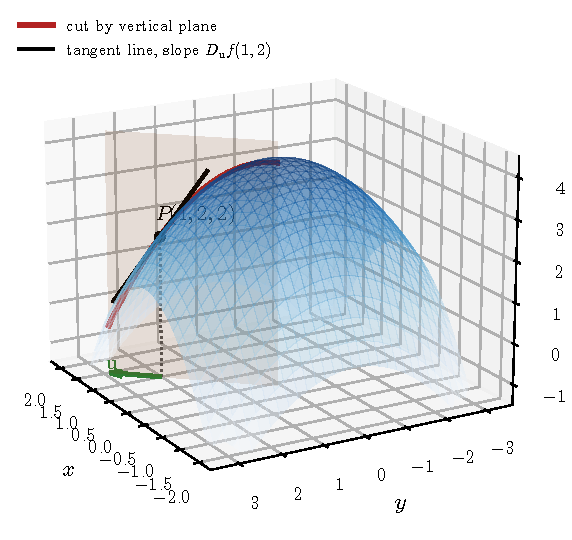
\includegraphics[width=0.66\linewidth]{surface_slice}
  \caption{The surface $z=4-x^2-\tfrac14y^2$ of Slides, Example~6.1, cut by the
  vertical plane through $(1,2)$ in the direction
  $\vu=\ip{\cos\frac\pi3,\sin\frac\pi3}$. The slope of the black tangent line is
  $\Du f(1,2)=-1-\frac{\sqrt3}{2}\approx-1.87$: walking in direction $\vu$ you go
  \emph{downhill}.}
  \label{fig:surface-slice}
\end{figure}

\subsection{Definition}

If we move from $(x_0,y_0)$ a distance $h$ in the direction of the \emph{unit}
vector $\vu=\ip{a,b}$, we arrive at $(x_0+ha,\,y_0+hb)$. Comparing the change
in $f$ with the distance $h$ travelled gives the following definition.

\begin{definition}[Directional derivative; Slides]\label{def:Du}
The \emph{directional derivative} of $f$ at $(x_0,y_0)$ in the direction of the
unit vector $\vu=\ip{a,b}$ is
\[
  \Du f(x_0,y_0)=\lim_{h\to0}\frac{f(x_0+ha,\;y_0+hb)-f(x_0,y_0)}{h},
\]
if this limit exists.
\end{definition}

\begin{remark}[Special cases]\label{rem:special}
With $\vu=\vi=\ip{1,0}$ the definition becomes the definition of $f_x$; with
$\vu=\vj=\ip{0,1}$ it becomes $f_y$. So
\[
  D_{\vi}f=f_x,\qquad D_{\vj}f=f_y .
\]
Partial derivatives are directional derivatives in two special directions.
\end{remark}

\begin{remark}[Why a \emph{unit} vector?]
The denominator $h$ is the distance travelled only because $\norm{\vu}=1$. If
$\vu$ had length $2$, moving ``$h$ units of $\vu$'' would cover a distance $2h$,
and the quotient would be twice the true slope. A directional derivative is a
rate of change \emph{per unit distance}, so the direction must always be
given by a unit vector.
\end{remark}

\begin{example}[Directional derivative from the definition]\label{ex:by-def}
Use Definition~\ref{def:Du} to compute $\Du f(1,2)$ for $f(x,y)=x^2-xy$ and
$\vu=\ip{\tfrac35,\tfrac45}$.
\end{example}
\begin{solution}
\step{1}{Check $\vu$ is a unit vector.} $\left(\frac35\right)^2+\left(\frac45\right)^2=\frac{9+16}{25}=1$.\checkok
\step{2}{The moved point.} $(x_0+ha,\,y_0+hb)=\left(1+\tfrac35h,\;2+\tfrac45h\right)$.
\step{3}{Evaluate $f$ there.}
\begin{align*}
f\!\left(1+\tfrac35h,\,2+\tfrac45h\right)
&=\left(1+\tfrac35h\right)^2-\left(1+\tfrac35h\right)\left(2+\tfrac45h\right)\\
&=\left(1+\tfrac65h+\tfrac{9}{25}h^2\right)-\left(2+\tfrac45h+\tfrac65h+\tfrac{12}{25}h^2\right)\\
&=-1-\tfrac45h-\tfrac{3}{25}h^2 .
\end{align*}
\step{4}{Difference quotient.} Since $f(1,2)=1-2=-1$,
\[
\frac{f(1+\frac35h,2+\frac45h)-f(1,2)}{h}=\frac{-\frac45h-\frac{3}{25}h^2}{h}=-\frac45-\frac{3}{25}h .
\]
\step{5}{Limit.} $\Du f(1,2)=\displaystyle\lim_{h\to0}\left(-\frac45-\frac{3}{25}h\right)=-\frac45.$

We will confirm this in one line with the formula of the next section.
\end{solution}

\subsection{The formula for the directional derivative}

Computing limits every time is slow. For differentiable functions there is a
formula in terms of the partial derivatives.

\begin{theorem}[Slides]\label{thm:Du-formula}
If $f$ is a differentiable function of $x$ and $y$, then $f$ has a directional
derivative in the direction of any unit vector $\vu=\ip{a,b}$ and
\[
  \boxed{\;\Du f(x,y)=f_x(x,y)\,a+f_y(x,y)\,b\;}
\]
\end{theorem}

\begin{proof}
Fix $(x_0,y_0)$ and define a function of one variable
\[
  g(h)=f(x_0+ha,\;y_0+hb).
\]
By the definition of the derivative of $g$ at $0$,
\[
  g'(0)=\lim_{h\to0}\frac{g(h)-g(0)}{h}
       =\lim_{h\to0}\frac{f(x_0+ha,y_0+hb)-f(x_0,y_0)}{h}=\Du f(x_0,y_0).
\]
On the other hand, $g(h)=f(x(h),y(h))$ with $x(h)=x_0+ha$ and $y(h)=y_0+hb$,
so $x'(h)=a$ and $y'(h)=b$. Since $f$ is differentiable, the chain rule
(Theorem~\ref{thm:chain}) gives
\[
  g'(h)=f_x(x(h),y(h))\,a+f_y(x(h),y(h))\,b .
\]
Putting $h=0$: $g'(0)=f_x(x_0,y_0)\,a+f_y(x_0,y_0)\,b$. Comparing the two
expressions for $g'(0)$ proves the formula.
\end{proof}

\begin{corollary}[Angle form; Slides]\label{cor:angle}
If the unit vector $\vu$ makes an angle $\theta$ with the positive $x$-axis,
then $\vu=\ip{\cos\theta,\sin\theta}$ and
\[
  \Du f(x,y)=f_x(x,y)\cos\theta+f_y(x,y)\sin\theta .
\]
\end{corollary}

\textbf{Check on Example~\ref{ex:by-def}.} $f_x=2x-y$ and $f_y=-x$ are
continuous, so $f$ is differentiable; at $(1,2)$, $f_x=0$, $f_y=-1$, hence
$\Du f(1,2)=0\cdot\frac35+(-1)\cdot\frac45=-\frac45$, as before.\checkok

\begin{remark}[Reversing direction]
Since $-\vu=\ip{-a,-b}$, the formula gives $D_{-\vu}f=-\Du f$: walking the
opposite way, uphill becomes downhill at the same rate.
\end{remark}

\begin{strategy}{Strategy (computing $\Du f(x_0,y_0)$).}
\begin{enumerate}
  \item Compute $f_x$ and $f_y$; note they are continuous, so $f$ is
        differentiable and Theorem~\ref{thm:Du-formula} applies.
  \item Get a \textbf{unit} vector $\vu=\ip{a,b}$:
        \begin{itemize}
          \item from an angle $\theta$: $\vu=\ip{\cos\theta,\sin\theta}$;
          \item from a vector $\vv$: $\vu=\vv/\norm{\vv}$;
          \item ``from $P$ towards $Q$'': $\vu=\vecPQ/\norm{\vecPQ}$.
        \end{itemize}
  \item Optionally write the general formula $\Du f(x,y)=f_x a+f_y b$.
  \item Evaluate at $(x_0,y_0)$. Interpret the sign: positive means $f$ increases
        in that direction, negative means it decreases.
\end{enumerate}
\end{strategy}

\subsection{Worked examples}

\begin{example}[Slides, Example 6.1]\label{ex:6.1}
Find the directional derivative of $f(x,y)=4-x^2-\tfrac14y^2$ at $(1,2)$ in the
direction of $\vu=\left(\cos\tfrac\pi3\right)\vi+\left(\sin\tfrac\pi3\right)\vj$.
\end{example}
\begin{solution}
\step{1}{Partial derivatives.} $f_x=-2x$ and $f_y=-\tfrac12y$. These are
continuous (polynomials), hence $f$ is differentiable.
\step{2}{General directional derivative.} By Corollary~\ref{cor:angle},
\[
  \Du f(x,y)=-2x\cos\theta-\tfrac12y\sin\theta .
\]
\step{3}{Substitute $\theta=\frac\pi3$, $x=1$, $y=2$.}
\[
  \Du f(1,2)=-2(1)\left(\tfrac12\right)-\tfrac12(2)\left(\tfrac{\sqrt3}{2}\right)
  =-1-\frac{\sqrt3}{2}=-\frac{2+\sqrt3}{2}\approx-1.866 .
\]
Interpretation: moving from $(1,2)$ in the direction $60^\circ$ above the
positive $x$-axis, the height of the hill decreases at about $1.87$ units of
height per unit of horizontal distance (Figure~\ref{fig:surface-slice}).
\end{solution}

\interactive{\desmosTD}{Open in Desmos 3D} and paste \texttt{z=4-x\^{}2-y\^{}2/4};
add the line \texttt{(1+t/2, 2+t*sqrt(3)/2, 2-(1+sqrt(3)/2)t)} with
$-1\le t\le1$ to see the tangent line of Figure~\ref{fig:surface-slice}.

\begin{example}[Slides, Example 6.2]\label{ex:6.2}
Find the directional derivative of $f(x,y)=x^2\sin2y$ at $\left(1,\tfrac\pi2\right)$
in the direction of $\vv=3\vi-4\vj$.
\end{example}
\begin{solution}
\step{1}{Partial derivatives.} $f_x=2x\sin2y$ and (chain rule)
$f_y=x^2\cdot\cos2y\cdot2=2x^2\cos2y$. Both are continuous, hence $f$ is
differentiable and
\[
  \Du f(x,y)=(2x\sin2y)\,a+(2x^2\cos2y)\,b,\qquad\text{where }\ip{a,b}=\frac{\vv}{\norm{\vv}} .
\]
\step{2}{Unit vector.} $\vv$ is \emph{not} a unit vector:
\[
  \ip{a,b}=\frac{\ip{3,-4}}{\sqrt{3^2+4^2}}=\ip{\tfrac35,-\tfrac45}.
\]
\step{3}{General formula.}
\[
  \Du f(x,y)=\tfrac35(2x\sin2y)-\tfrac45(2x^2\cos2y)=\tfrac65x\sin2y-\tfrac85x^2\cos2y .
\]
\step{4}{Evaluate.} At $\left(1,\frac\pi2\right)$: $\sin\pi=0$ and $\cos\pi=-1$, so
\[
  \Du f\!\left(1,\tfrac\pi2\right)=\tfrac65(1)(0)-\tfrac85(1)^2(-1)=\frac85 .
\]
\end{solution}

\begin{warning}[The most common mistake]
Using $\vv=\ip{3,-4}$ itself instead of the unit vector would give
$f_x\cdot3+f_y\cdot(-4)=0+(-2)(-4)=8$, which is $\norm{\vv}=5$ times too big.
Always normalize first.
\end{warning}

\begin{example}\label{ex:pi6}
Find $\Du f(1,2)$ for $f(x,y)=x^3-3xy+4y^2$, where $\vu$ is the unit vector
given by the angle $\theta=\frac\pi6$.
\end{example}
\begin{solution}
\step{1}{Partials.} $f_x=3x^2-3y$, $f_y=-3x+8y$ (continuous).
\step{2}{At $(1,2)$.} $f_x(1,2)=3-6=-3$ and $f_y(1,2)=-3+16=13$.
\step{3}{Angle form.} $\cos\frac\pi6=\frac{\sqrt3}{2}$, $\sin\frac\pi6=\frac12$:
\[
  \Du f(1,2)=-3\cdot\frac{\sqrt3}{2}+13\cdot\frac12=\frac{13-3\sqrt3}{2}\approx3.90 .
\]
\end{solution}

\begin{example}[Slides, Example 6.4]\label{ex:6.4}
Find the directional derivative of $f(x,y)=3x^2-2y^2$ at the point
$\left(-\tfrac34,0\right)$ in the direction from $P\left(-\tfrac34,0\right)$ to
$Q(0,1)$.
\end{example}
\begin{solution}
\step{1}{Differentiability.} $f_x=6x$ and $f_y=-4y$ are continuous, so $f$ is
differentiable.
\step{2}{Direction vector.}
$\vecPQ=\ip{0-\left(-\tfrac34\right),\;1-0}=\ip{\tfrac34,1}$.
\step{3}{Unit vector.}
\[
  \vu=\frac{\vecPQ}{\norm{\vecPQ}}=\frac{\ip{\frac34,1}}{\sqrt{\left(\frac34\right)^2+1^2}}
  =\frac{\ip{\frac34,1}}{\frac54}=\ip{\tfrac35,\tfrac45}.
\]
\step{4}{Partials at the point.} $f_x\left(-\tfrac34,0\right)=6\left(-\tfrac34\right)=-\tfrac92$ and
$f_y\left(-\tfrac34,0\right)=0$.
\step{5}{Directional derivative.}
\[
  \Du f\left(-\tfrac34,0\right)=-\frac92\cdot\frac35+0\cdot\frac45=-\frac{27}{10}.
\]
\end{solution}

\begin{remark}
On the slide the last line reads ``the directional derivative at $(-3/2,0)$'';
this is a typo for $(-\tfrac34,0)$, the point actually used in the
computation. The slide writes the answer as $\grad f\cdot\vu$; this
dot-product form is the subject of Chapter~\ref{ch:gradient}.
\end{remark}

\begin{example}[An applied interpretation]\label{ex:temp}
The temperature (in $^\circ$C) on a metal plate is $T(x,y)=100-x^2-2y^2$, where
$x,y$ are in metres. An ant at $(3,1)$ starts walking towards the point
$(5,2)$. At what rate does the temperature change as it starts to walk?
\end{example}
\begin{solution}
\step{1}{Partials at $(3,1)$.} $T_x=-2x=-6$ and $T_y=-4y=-4$.
\step{2}{Direction.} $\vecPQ=\ip{5-3,\,2-1}=\ip{2,1}$, $\norm{\vecPQ}=\sqrt5$,
$\vu=\ip{\tfrac{2}{\sqrt5},\tfrac{1}{\sqrt5}}$.
\step{3}{Rate.}
\[
  \Du T(3,1)=-6\cdot\frac{2}{\sqrt5}-4\cdot\frac{1}{\sqrt5}=-\frac{16}{\sqrt5}=-\frac{16\sqrt5}{5}\approx-7.16 .
\]
The temperature \emph{drops} by about $7.16\,^\circ$C per metre walked, at the
instant the ant starts. (Units of $\Du T$: units of $T$ per unit of distance.)
\end{solution}

\subsection{Functions of three variables}

Everything above extends verbatim to $w=f(x,y,z)$.

\begin{definition}
For a unit vector $\vu=\ip{a,b,c}$,
\[
  \Du f(x_0,y_0,z_0)=\lim_{h\to0}\frac{f(x_0+ha,\,y_0+hb,\,z_0+hc)-f(x_0,y_0,z_0)}{h}.
\]
\end{definition}

\begin{theorem}\label{thm:Du3}
If $f(x,y,z)$ is differentiable and $\vu=\ip{a,b,c}$ is a unit vector, then
\[
  \Du f(x,y,z)=f_x(x,y,z)\,a+f_y(x,y,z)\,b+f_z(x,y,z)\,c .
\]
\end{theorem}
The proof is identical to that of Theorem~\ref{thm:Du-formula}, using the
three-variable chain rule.

\begin{example}\label{ex:3var}
Find the directional derivative of $f(x,y,z)=x\sin(yz)$ at $(1,3,0)$ in the
direction of $\vv=\vi+2\vj-\vk$.
\end{example}
\begin{solution}
\step{1}{Partials.} $f_x=\sin(yz)$, $f_y=xz\cos(yz)$, $f_z=xy\cos(yz)$, all continuous.
\step{2}{At $(1,3,0)$.} $yz=0$, so $\sin(yz)=0$ and $\cos(yz)=1$:
\[
  f_x=0,\qquad f_y=(1)(0)(1)=0,\qquad f_z=(1)(3)(1)=3 .
\]
\step{3}{Unit vector.} $\norm{\vv}=\sqrt{1+4+1}=\sqrt6$, so
$\vu=\ip{\tfrac{1}{\sqrt6},\tfrac{2}{\sqrt6},-\tfrac{1}{\sqrt6}}$.
\step{4}{Directional derivative.}
\[
  \Du f(1,3,0)=0\cdot\tfrac{1}{\sqrt6}+0\cdot\tfrac{2}{\sqrt6}+3\cdot\left(-\tfrac{1}{\sqrt6}\right)
  =-\frac{3}{\sqrt6}=-\frac{\sqrt6}{2}\approx-1.22 .
\]
\end{solution}

% =====================================================================
\section{The Gradient Vector}\label{ch:gradient}
% =====================================================================

\subsection{Definition}

The formula of Theorem~\ref{thm:Du-formula} has the shape of a dot product
(Slides, \emph{Gradient Vectors}):
\[
  \Du f(x,y)=f_x(x,y)\,a+f_y(x,y)\,b=\ip{f_x(x,y),\,f_y(x,y)}\cdot\ip{a,b}
  =\ip{f_x(x,y),\,f_y(x,y)}\cdot\vu .
\]
The first vector depends only on $f$ and the point, not on the direction. It
occurs so often that it gets a name.

\begin{definition}[Gradient; Slides]\label{def:grad}
If $f$ is a function of two variables $x$ and $y$, the \emph{gradient} of $f$
is the vector function $\grad f$ (read ``del $f$'', also written
$\operatorname{grad}f$) defined by
\[
  \grad f(x,y)=\ip{f_x(x,y),\,f_y(x,y)}=\pd{f}{x}\,\vi+\pd{f}{y}\,\vj .
\]
For a function of three variables,
$\grad f(x,y,z)=\ip{f_x,\,f_y,\,f_z}=\pd fx\vi+\pd fy\vj+\pd fz\vk$.
\end{definition}

\begin{keybox}{Directional derivative as a dot product}
If $f$ is differentiable and $\vu$ is a \emph{unit} vector, then
\[
  \Du f=\grad f\cdot\vu
\]
in two or three variables (Theorems~\ref{thm:Du-formula} and~\ref{thm:Du3}).
\end{keybox}

Note the types: $f$ is a scalar function, $\grad f$ is a \emph{vector}, and
$\Du f=\grad f\cdot\vu$ is again a \emph{scalar}. Writing $\grad f$ for a number
or $\Du f$ as a vector are common, costly mistakes.

\begin{example}[Slides, Example 6.3]\label{ex:6.3}
Find the gradient of $f(x,y)=y\ln x+xy^2$ at the point $(1,2)$.
\end{example}
\begin{solution}
\step{1}{Partial derivatives.} $f_x=\dfrac{y}{x}+y^2$ and $f_y=\ln x+2xy$.
\step{2}{Gradient.} $\grad f(x,y)=\ip{\dfrac yx+y^2,\;\ln x+2xy}$.
\step{3}{At $(1,2)$.}
\[
  \grad f(1,2)=\ip{\tfrac21+2^2,\;\ln1+2(1)(2)}=\ip{6,4}.
\]
\end{solution}

\begin{example}[Slides, Example 6.4 via the gradient]
Redo Example~\ref{ex:6.4} using $\Du f=\grad f\cdot\vu$.
\end{example}
\begin{solution}
$\grad f(x,y)=\ip{6x,-4y}$, so $\grad f\left(-\tfrac34,0\right)=\ip{-\tfrac92,0}$; with
$\vu=\ip{\tfrac35,\tfrac45}$,
\[
  \Du f\left(-\tfrac34,0\right)=\ip{-\tfrac92,0}\cdot\ip{\tfrac35,\tfrac45}=-\frac{27}{10}.
\]
\emph{Caution:} the slide prints the middle step as $\ip{-9,0}$, but
$6\left(-\frac34\right)=-\frac92$, not $-9$. With $\ip{-9,0}$ one would get
$-\frac{27}{5}$; the slide's final answer $-\frac{27}{10}$ is the correct one,
coming from $\ip{-\frac92,0}$.
\end{solution}

\subsection{Maximizing the directional derivative}

Let $\theta$ be the angle between $\grad f$ and the unit vector $\vu$. By the
geometric form of the dot product (Slides),
\[
  \Du f=\grad f\cdot\vu=\norm{\grad f}\,\norm{\vu}\cos\theta=\norm{\grad f}\cos\theta,
\]
because $\norm{\vu}=1$. Everything about the size of $\Du f$ is now controlled
by the single number $\cos\theta\in[-1,1]$ (Figure~\ref{fig:angle}).

\begin{figure}[H]
\centering
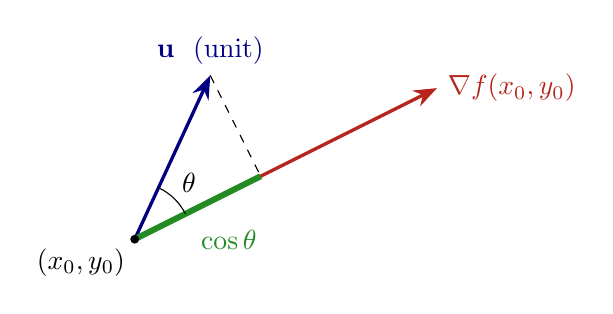
\begin{tikzpicture}[scale=1.6,>=Stealth]
  \draw[->,very thick,BrickRed] (0,0) -- (2.4,1.2) node[right]{$\grad f(x_0,y_0)$};
  \draw[->,very thick,NavyBlue] (0,0) -- (0.6,1.3) node[above]{$\vu$ \ (unit)};
  \draw[dashed] (0.6,1.3) -- (1.0,0.5);
  \draw[line width=2.2pt,ForestGreen] (0,0) -- (1.0,0.5);
  \node[ForestGreen,below right] at (0.45,0.15) {$\cos\theta$};
  \draw ({0.45*cos(26.57)},{0.45*sin(26.57)}) arc[start angle=26.57,end angle=65.22,radius=0.45];
  \node at ({0.62*cos(46)},{0.62*sin(46)}) {$\theta$};
  \fill (0,0) circle (1pt) node[below left]{$(x_0,y_0)$};
\end{tikzpicture}
\caption{$\Du f=\norm{\grad f}\cos\theta$. The green segment is the projection
of the unit vector $\vu$ onto the direction of $\grad f$; it has signed length
$\cos\theta$. It is longest when $\vu$ points along $\grad f$.}
\label{fig:angle}
\end{figure}

\begin{theorem}[Maximum rate of change; Slides]\label{thm:max}
Let $f$ be differentiable at $P$ with $\grad f(P)\neq\vzero$. Then, as $\vu$
ranges over all unit vectors:
\begin{enumerate}[label=(\alph*)]
  \item the \textbf{maximum} value of $\Du f(P)$ is $\norm{\grad f(P)}$, attained
        exactly when $\vu$ points in the direction of $\grad f(P)$, i.e.
        $\vu=\grad f(P)/\norm{\grad f(P)}$ ($\theta=0$);
  \item the \textbf{minimum} value is $-\norm{\grad f(P)}$, attained when $\vu$
        points in the direction of $-\grad f(P)$ ($\theta=\pi$);
  \item $\Du f(P)=0$ exactly when $\vu\perp\grad f(P)$ ($\theta=\frac\pi2$);
  \item every value in $\left[-\norm{\grad f(P)},\;\norm{\grad f(P)}\right]$ is
        attained, and no other value is.
\end{enumerate}
If $\grad f(P)=\vzero$, then $\Du f(P)=0$ for every $\vu$.
\end{theorem}

\begin{proof}
Since $-1\le\cos\theta\le1$, we get
$-\norm{\grad f}\le\norm{\grad f}\cos\theta\le\norm{\grad f}$. The value
$\cos\theta=1$ occurs only for $\theta=0$, i.e. $\vu$ has the direction of
$\grad f$; $\cos\theta=-1$ only for $\theta=\pi$; $\cos\theta=0$ only for
$\theta=\frac\pi2$. As $\theta$ varies continuously from $0$ to $\pi$,
$\cos\theta$ takes every value in $[-1,1]$, giving (d).
\end{proof}

\begin{keybox}{In words}
The gradient $\grad f$ points in the direction in which $f$ \emph{increases
most rapidly}, and its length $\norm{\grad f}$ is that maximum rate of
increase. $-\grad f$ is the direction of fastest decrease. Directions
perpendicular to $\grad f$ are directions of no instantaneous change.
\end{keybox}

\begin{example}\label{ex:xey}
Let $f(x,y)=xe^y$.
(a) Find the rate of change of $f$ at $P(2,0)$ in the direction from $P$ to
$Q\left(\tfrac12,2\right)$.
(b) In what direction does $f$ have the maximum rate of change at $P$? What is
this maximum rate?
\end{example}
\begin{solution}
\step{1}{Gradient.} $\grad f(x,y)=\ip{e^y,\;xe^y}$, so $\grad f(2,0)=\ip{1,2}$.

\textbf{(a)} $\vecPQ=\ip{\tfrac12-2,\;2-0}=\ip{-\tfrac32,2}$. Scale by $2$:
$\ip{-3,4}$ has the same direction and length $5$, so $\vu=\ip{-\tfrac35,\tfrac45}$.
\[
  \Du f(2,0)=\ip{1,2}\cdot\ip{-\tfrac35,\tfrac45}=-\tfrac35+\tfrac85=1 .
\]

\textbf{(b)} By Theorem~\ref{thm:max}, $f$ increases fastest in the direction of
$\grad f(2,0)=\ip{1,2}$ (unit vector $\ip{\tfrac{1}{\sqrt5},\tfrac{2}{\sqrt5}}$),
and the maximum rate is $\norm{\ip{1,2}}=\sqrt5\approx2.24$.

Figure~\ref{fig:du-theta} plots $\Du f(2,0)=\cos\theta+2\sin\theta$ against the
angle $\theta$ of $\vu$: it oscillates between $-\sqrt5$ and $\sqrt5$, exactly
as Theorem~\ref{thm:max} predicts.
\end{solution}

\begin{figure}[H]
  \centering
  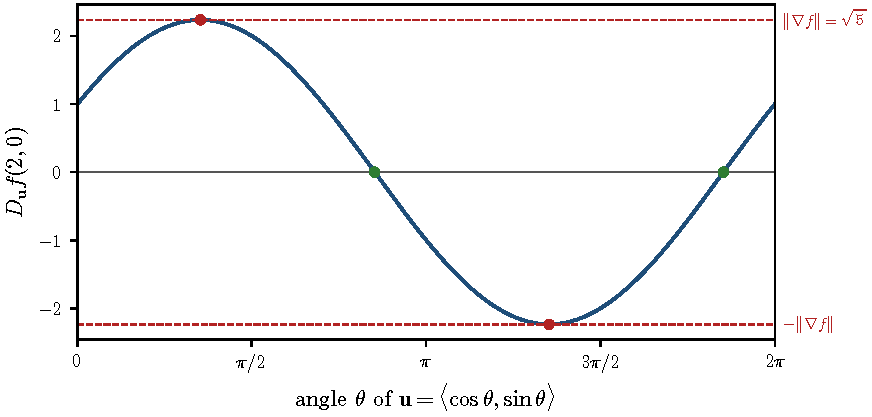
\includegraphics[width=0.78\linewidth]{du_vs_theta}
  \caption{$\Du f(2,0)$ for $f=xe^y$ as $\vu$ turns once around the circle. Red:
  maximum $\sqrt5$ at $\theta=\arctan2$ (the direction of $\grad f$) and minimum
  $-\sqrt5$ half a turn later. Green: the two directions perpendicular to
  $\grad f$, where the rate is $0$.}
  \label{fig:du-theta}
\end{figure}

\subsection{The trio activity, solved}

\begin{example}[Slides, Activity (by trio)]\label{ex:trio}
Let $f(x,y)=200e^{-x^2-3y^2}$.
\begin{enumerate}[label=(\alph*)]
  \item Find the directional derivative of $f$ at $P(4,-1)$ in the direction toward $Q(7,3)$.
  \item Determine the direction in which $f$ increases most rapidly at $P$.
  \item Find the maximum rate of increase of $f$ at $P$.
\end{enumerate}
\end{example}
\begin{solution}
\step{1}{Gradient.} By the chain rule,
\[
  f_x=200e^{-x^2-3y^2}\cdot(-2x)=-400x\,e^{-x^2-3y^2},\qquad
  f_y=200e^{-x^2-3y^2}\cdot(-6y)=-1200y\,e^{-x^2-3y^2}.
\]
These are continuous, so $f$ is differentiable.
\step{2}{At $P(4,-1)$.} The exponent is $-16-3=-19$, so
\[
  \grad f(4,-1)=\ip{-1600e^{-19},\;1200e^{-19}}=400e^{-19}\ip{-4,3}.
\]
\textbf{(a)} $\vecPQ=\ip{7-4,\;3-(-1)}=\ip{3,4}$, $\norm{\vecPQ}=5$,
$\vu=\ip{\tfrac35,\tfrac45}$. Hence
\[
  \Du f(4,-1)=400e^{-19}\ip{-4,3}\cdot\ip{\tfrac35,\tfrac45}
  =400e^{-19}\left(-\tfrac{12}{5}+\tfrac{12}{5}\right)=0 .
\]
\textbf{(b)} The direction of $\grad f(4,-1)$, i.e. of $\ip{-4,3}$; as a unit
vector, $\ip{-\tfrac45,\tfrac35}$.

\textbf{(c)} $\norm{\grad f(4,-1)}=400e^{-19}\sqrt{16+9}=2000e^{-19}\approx1.12\times10^{-5}$.

\textbf{Why is (a) zero?} The level curves of $f$ are the ellipses
$x^2+3y^2=c$. The one through $P$ is $x^2+3y^2=19$, and the direction
$\ip{3,4}$ is tangent to it at $P$ (it is perpendicular to $\grad f(P)\parallel\ip{-4,3}$).
Moving along a level curve, $f$ does not change to first order, so the rate is
$0$ (Theorem~\ref{thm:max}(c); Figure~\ref{fig:trio}).
\end{solution}

\begin{figure}[H]
  \centering
  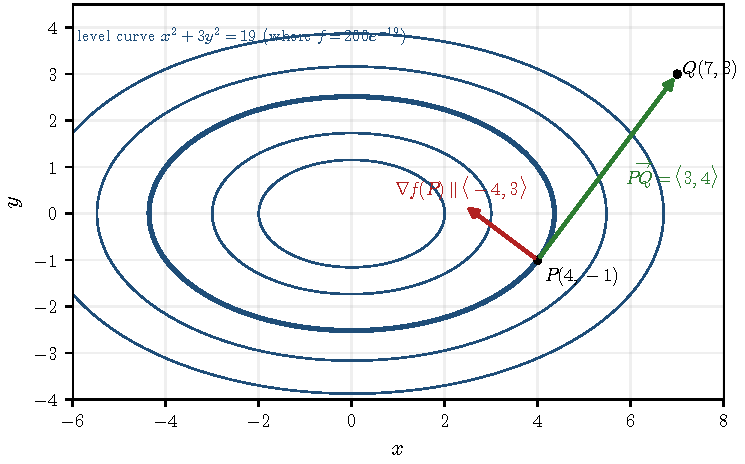
\includegraphics[width=0.72\linewidth]{trio_activity}
  \caption{Trio activity. $\protect\vecPQ$ (green) is tangent to the level
  curve through $P$, so it is perpendicular to the gradient (red) and the
  directional derivative is $0$.}
  \label{fig:trio}
\end{figure}

\subsection{More examples}

\begin{example}[Three variables]\label{ex:temp3}
The temperature at $(x,y,z)$ is $T(x,y,z)=\dfrac{80}{1+x^2+2y^2+3z^2}$
($^\circ$C, metres). In which direction does the temperature increase fastest at
$(1,1,-2)$? What is the maximum rate of increase?
\end{example}
\begin{solution}
\step{1}{Gradient.} Write $T=80\,D^{-1}$ with $D=1+x^2+2y^2+3z^2$. Then
$T_x=-80D^{-2}\cdot2x$, etc.:
\[
  \grad T=\frac{-80}{(1+x^2+2y^2+3z^2)^2}\ip{2x,\;4y,\;6z}.
\]
\step{2}{At $(1,1,-2)$.} $D=1+1+2+12=16$, so
\[
  \grad T(1,1,-2)=\frac{-80}{256}\ip{2,4,-12}=\frac{-5}{16}\ip{2,4,-12}=\frac58\ip{-1,-2,6}.
\]
\step{3}{Answer.} The temperature increases fastest in the direction of
$\ip{-1,-2,6}$ (unit vector $\frac{1}{\sqrt{41}}\ip{-1,-2,6}$); the maximum rate is
\[
  \norm{\grad T(1,1,-2)}=\frac58\sqrt{1+4+36}=\frac{5\sqrt{41}}{8}\approx4.00\ ^\circ\text{C/m}.
\]
\end{solution}

\begin{example}[Finding directions with a prescribed rate]\label{ex:prescribed}
Let $f(x,y)=x^2y$ and $P(1,2)$.
(a) Find all unit vectors $\vu$ with $\Du f(P)=1$.
(b) Find all $\vu$ with $\Du f(P)=0$.
(c) Is there a direction with $\Du f(P)=5$?
\end{example}
\begin{solution}
\step{1}{Gradient.} $\grad f=\ip{2xy,\,x^2}$, so $\grad f(1,2)=\ip{4,1}$ and
$\norm{\grad f(1,2)}=\sqrt{17}\approx4.12$.

\textbf{(a)} Let $\vu=\ip{a,b}$. We need
\[
  4a+b=1\qquad\text{and}\qquad a^2+b^2=1 .
\]
From the first, $b=1-4a$. Substituting: $a^2+(1-4a)^2=1\iff17a^2-8a=0\iff a(17a-8)=0$.
\begin{itemize}
  \item $a=0\Rightarrow b=1$: $\vu=\ip{0,1}$.
  \item $a=\frac{8}{17}\Rightarrow b=1-\frac{32}{17}=-\frac{15}{17}$: $\vu=\ip{\frac{8}{17},-\frac{15}{17}}$.
\end{itemize}
Check: $4(0)+1=1$\checkok; $\frac{32}{17}-\frac{15}{17}=1$\checkok. Two directions,
symmetric about $\grad f$, as expected from $\Du f=\sqrt{17}\cos\theta$, where
$\cos\theta=1/\sqrt{17}$ has two solutions $\pm\theta$.

\textbf{(b)} $\vu\perp\ip{4,1}$: $\vu=\pm\frac{1}{\sqrt{17}}\ip{1,-4}$.

\textbf{(c)} No: $5>\sqrt{17}=\norm{\grad f(P)}$, the largest possible value
(Theorem~\ref{thm:max}(d)).
\end{solution}

\subsection{Rules for gradients}

Because partial derivatives obey the usual rules, so does $\grad$. For
differentiable $f,g$ and constants $\alpha,\beta$:
\[
  \grad(\alpha f+\beta g)=\alpha\grad f+\beta\grad g,\qquad
  \grad(fg)=f\grad g+g\grad f,\qquad
  \grad\!\left(\frac fg\right)=\frac{g\grad f-f\grad g}{g^2},
\]
and for a differentiable one-variable function $F$, the chain rule gives
$\grad\big(F(f)\big)=F'(f)\,\grad f$.

\begin{example}[Gradient of distance]\label{ex:grad-r}
Let $r=\sqrt{x^2+y^2+z^2}$ be the distance from the origin and
$\vx=\ip{x,y,z}$. Show that $\grad r=\dfrac{\vx}{r}$ and
$\grad\!\left(\dfrac1r\right)=-\dfrac{\vx}{r^3}$ for $\vx\neq\vzero$.
\end{example}
\begin{solution}
\step{1}{$\grad r$.} $\pd rx=\dfrac{1}{2\sqrt{x^2+y^2+z^2}}\cdot2x=\dfrac xr$, and
likewise $\pd ry=\dfrac yr$, $\pd rz=\dfrac zr$. So $\grad r=\dfrac1r\ip{x,y,z}=\dfrac{\vx}{r}$:
a unit vector pointing directly away from the origin (distance grows fastest
moving radially outward, at rate $1$).
\step{2}{$\grad(1/r)$.} With $F(s)=1/s$, $F'(s)=-1/s^2$, the chain rule gives
\[
  \grad\!\left(\frac1r\right)=-\frac1{r^2}\,\grad r=-\frac{1}{r^2}\cdot\frac{\vx}{r}=-\frac{\vx}{r^3}.
\]
This vector field, pointing toward the origin with magnitude $1/r^2$, is the
shape of Newton's gravitational field; it reappears in Lecture Notes No.~7.
\end{solution}

\begin{remark}[Looking ahead]
$\grad f$ assigns a vector to every point of the domain, so it is a
\emph{vector field}: the \emph{gradient field} of $f$. Vector fields, gradient
fields and their ``potential functions'' are the topic of Lecture Notes
No.~7 (Slides~7, \emph{Vector Calculus}).
\end{remark}

% =====================================================================
\section{Geometry of the Gradient}\label{ch:geometry}
% =====================================================================

The slides prove that $\grad f$ points in the direction of fastest increase.
This chapter adds the companion fact that makes gradients so useful in
geometry: the gradient is \emph{perpendicular to level curves and level
surfaces}. It explains Figure~\ref{fig:trio} and gives a quick way to find
tangent lines and tangent planes. (This material extends the slides; it is
standard in the course textbook and frequently appears as part of a gradient
problem.)

\subsection{The gradient is perpendicular to level curves}

\begin{theorem}\label{thm:grad-perp}
Let $f$ be differentiable and let $P(x_0,y_0)$ lie on the level curve
$f(x,y)=k$. If $\grad f(x_0,y_0)\neq\vzero$, then $\grad f(x_0,y_0)$ is
perpendicular to the level curve at $P$, i.e.\ to its tangent vector.
The same holds in three variables: $\grad f(x_0,y_0,z_0)$ is normal to the
level surface $f(x,y,z)=k$ through the point.
\end{theorem}

\begin{proof}
Let $\vr(t)=\ip{x(t),y(t)}$ be a differentiable parametrization of the level
curve with $\vr(t_0)=\ip{x_0,y_0}$. Since the curve lies in the level set,
$f(x(t),y(t))=k$ for all $t$. Differentiate both sides with respect to $t$
using the chain rule (Theorem~\ref{thm:chain}):
\[
  f_x\,x'(t)+f_y\,y'(t)=0,\qquad\text{i.e.}\qquad \grad f(\vr(t))\cdot\vr\,'(t)=0 .
\]
At $t=t_0$ this says $\grad f(x_0,y_0)\perp\vr\,'(t_0)$, the tangent vector.
For a level surface, apply the same argument to every curve on the surface
through the point: $\grad f$ is perpendicular to all their tangent vectors,
hence to the tangent plane.
\end{proof}

Combined with Theorem~\ref{thm:max}, this gives the familiar picture of a
contour map (Figure~\ref{fig:contour-gradient}): gradient vectors cross the
level curves at right angles, pointing ``uphill'', and they are longest where
the level curves are packed most tightly (where the surface is steepest).

\begin{figure}[H]
  \centering
  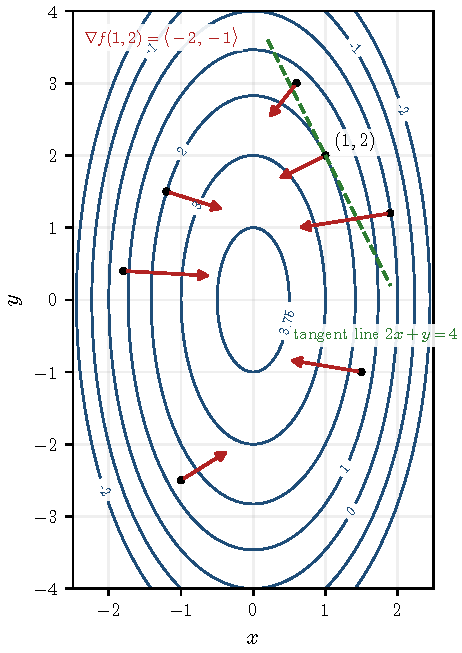
\includegraphics[width=0.62\linewidth]{contour_gradient}
  \caption{Level curves of $f(x,y)=4-x^2-\frac14y^2$ (labelled with their
  heights) and gradient vectors $\grad f=\ip{-2x,-\frac y2}$ (red, scaled by
  $0.35$). Each gradient is perpendicular to the level curve through its base
  point and points toward higher values. Green: the tangent line at $(1,2)$
  found in Example~\ref{ex:tangent-line}.}
  \label{fig:contour-gradient}
\end{figure}

\begin{example}[Tangent line to a level curve]\label{ex:tangent-line}
Find the tangent line at $(1,2)$ to the level curve of
$f(x,y)=4-x^2-\tfrac14y^2$ that passes through that point.
\end{example}
\begin{solution}
\step{1}{Which level curve?} $f(1,2)=4-1-1=2$, so the curve is
$4-x^2-\tfrac14y^2=2$, i.e. $x^2+\frac{y^2}{4}=2$.
\step{2}{Normal vector.} $\grad f(1,2)=\ip{-2(1),-\tfrac12(2)}=\ip{-2,-1}$ is
perpendicular to the curve at $(1,2)$.
\step{3}{Line through $(1,2)$ perpendicular to $\ip{-2,-1}$.}
\[
  -2(x-1)-1(y-2)=0\iff 2x+y=4 .
\]
\step{4}{Check by implicit differentiation.} $2x+\frac{y}{2}y'=0\Rightarrow
y'=-\frac{4x}{y}=-2$ at $(1,2)$, the slope of $y=4-2x$.\checkok
\end{solution}

\subsection{Tangent planes and normal lines to level surfaces}

\begin{definition}
Let $S$ be the level surface $F(x,y,z)=k$ and $P(x_0,y_0,z_0)$ a point of $S$
with $\grad F(P)\neq\vzero$.
\begin{itemize}
\item The \emph{tangent plane} to $S$ at $P$ is the plane through $P$ with
      normal vector $\grad F(P)$:
      \[
        F_x(P)(x-x_0)+F_y(P)(y-y_0)+F_z(P)(z-z_0)=0 .
      \]
\item The \emph{normal line} to $S$ at $P$ is the line through $P$ in the
      direction of $\grad F(P)$:
      \[
        x=x_0+F_x(P)\,t,\quad y=y_0+F_y(P)\,t,\quad z=z_0+F_z(P)\,t .
      \]
\end{itemize}
\end{definition}

\begin{example}[Tangent plane to an ellipsoid]\label{ex:ellipsoid}
Find the equations of the tangent plane and normal line at $(-2,1,-3)$ to the
ellipsoid $\dfrac{x^2}{4}+y^2+\dfrac{z^2}{9}=3$.
\end{example}
\begin{solution}
\step{1}{Set up $F$.} $F(x,y,z)=\dfrac{x^2}{4}+y^2+\dfrac{z^2}{9}$; the ellipsoid is
the level surface $F=3$. Check the point: $\frac44+1+\frac99=3$.\checkok
\step{2}{Gradient.} $\grad F=\ip{\dfrac x2,\;2y,\;\dfrac{2z}{9}}$, so
$\grad F(-2,1,-3)=\ip{-1,\;2,\;-\tfrac23}$.
\step{3}{Tangent plane.}
\[
  -1(x+2)+2(y-1)-\tfrac23(z+3)=0 .
\]
Multiplying by $-3$: $3(x+2)-6(y-1)+2(z+3)=0$, i.e.
$\boxed{3x-6y+2z+18=0}$.
\step{4}{Normal line.} $x=-2-t,\quad y=1+2t,\quad z=-3-\tfrac23t$.
\end{solution}

\begin{figure}[H]
  \centering
  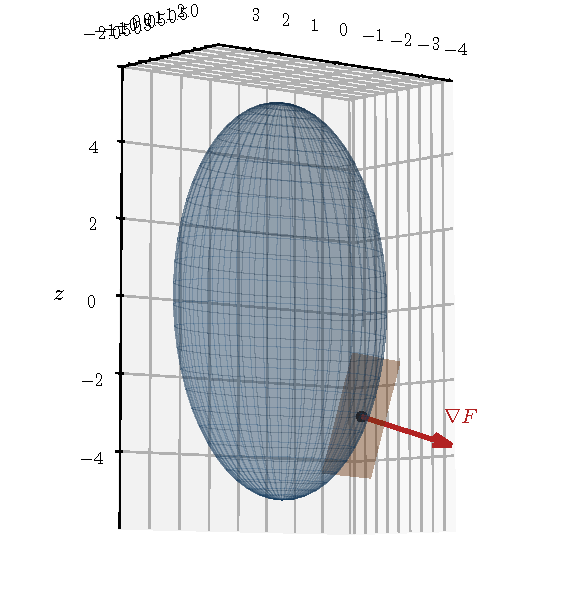
\includegraphics[width=0.5\linewidth]{ellipsoid_tangent_plane}
  \caption{The ellipsoid of Example~\ref{ex:ellipsoid}, a patch of its tangent
  plane at $(-2,1,-3)$, and the normal vector $\grad F(-2,1,-3)$.}
  \label{fig:ellipsoid}
\end{figure}

\begin{remark}[Graphs are level surfaces]
The graph $z=f(x,y)$ is the level surface $F(x,y,z)=f(x,y)-z=0$, and
$\grad F=\ip{f_x,f_y,-1}$. The tangent plane at $(x_0,y_0,z_0)$ is therefore
$f_x(x-x_0)+f_y(y-y_0)-(z-z_0)=0$, i.e.
\[
  z-z_0=f_x(x_0,y_0)(x-x_0)+f_y(x_0,y_0)(y-y_0),
\]
the usual tangent-plane formula for a graph.
\end{remark}

\begin{example}\label{ex:tp-graph}
Find the tangent plane to $z=4-x^2-\frac14y^2$ at $(1,2,2)$.
\end{example}
\begin{solution}
$f_x(1,2)=-2$, $f_y(1,2)=-1$, so $z-2=-2(x-1)-1(y-2)$, i.e. $2x+y+z=6$.
(Check: $2+2+2=6$.\checkok) Notice that the tangent line of
Figure~\ref{fig:surface-slice} lies in this plane: its points
$\left(1+\frac t2,\;2+\frac{\sqrt3}{2}t,\;2-\left(1+\frac{\sqrt3}{2}\right)t\right)$
satisfy $2x+y+z=6$ for every $t$.
\end{solution}

\subsection{Paths of steepest ascent}

A hiker who always walks in the direction of the gradient follows a
\emph{path of steepest ascent}. Its projection onto the $xy$-plane is a curve
whose tangent is parallel to $\grad f$ at every point, so it crosses every
level curve at right angles.

\begin{example}\label{ex:steepest}
For the hill $z=4-x^2-\frac14y^2$, find the path of steepest ascent (in the
$xy$-plane) starting at $(1,2)$.
\end{example}
\begin{solution}
\step{1}{Slope condition.} A curve $y=y(x)$ has tangent direction
$\ip{1,y'}$, which must be parallel to $\grad f=\ip{-2x,-\frac y2}$. Hence
\[
  \frac{\dd y}{\dd x}=\frac{f_y}{f_x}=\frac{-y/2}{-2x}=\frac{y}{4x}.
\]
\step{2}{Separate variables} (for $x,y>0$):
$\displaystyle\int\frac{\dd y}{y}=\int\frac{\dd x}{4x}\Rightarrow\ln y=\tfrac14\ln x+C
\Rightarrow y=Kx^{1/4}.$
\step{3}{Initial point.} $2=K\cdot1^{1/4}$, so $K=2$ and the path is
$y=2x^{1/4}$, travelled from $(1,2)$ toward the summit $(0,0)$ (the gradient
$\ip{-2,-1}$ at the start points toward decreasing $x$).
\end{solution}

\begin{figure}[H]
  \centering
  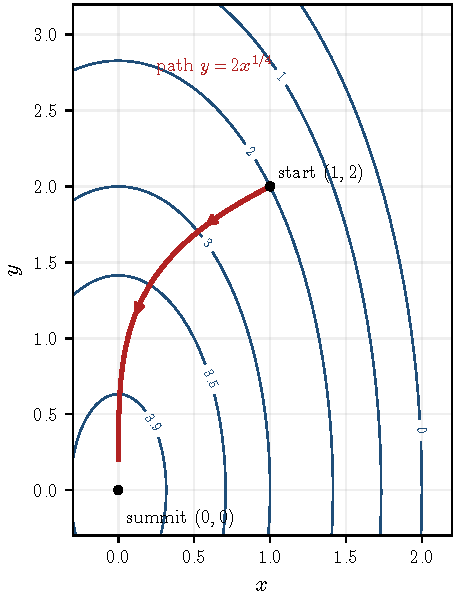
\includegraphics[width=0.48\linewidth]{steepest_ascent}
  \caption{The path of steepest ascent $y=2x^{1/4}$ from $(1,2)$ crosses every
  level curve at a right angle and climbs to the summit.}
  \label{fig:steepest}
\end{figure}

\subsection{What the gradient tells you}

\begin{center}
\renewcommand{\arraystretch}{1.35}
\begin{tabularx}{0.95\linewidth}{>{\raggedright\arraybackslash}p{0.38\linewidth}X}
\toprule
\textbf{Question at a point $P$} & \textbf{Answer in terms of $\grad f(P)$}\\
\midrule
Rate of change in direction $\vu$ ($\norm{\vu}=1$) & $\Du f(P)=\grad f(P)\cdot\vu$\\
Direction of fastest increase & $\grad f(P)$ \quad (unit: $\grad f/\norm{\grad f}$)\\
Fastest rate of increase & $\norm{\grad f(P)}$\\
Direction / rate of fastest decrease & $-\grad f(P)$, \ rate $-\norm{\grad f(P)}$\\
Directions of zero rate & $\vu\perp\grad f(P)$ (tangent to the level curve)\\
Normal to level curve / surface & $\grad f(P)$\\
Possible values of $\Du f(P)$ & exactly $\left[-\norm{\grad f(P)},\,\norm{\grad f(P)}\right]$\\
\bottomrule
\end{tabularx}
\end{center}

% =====================================================================
\section{Practice Problems with Complete Solutions}\label{ch:practice}
% =====================================================================

The problems follow the patterns of the slides: (i) $\Du f$ with the
direction given by an angle (Example~6.1), (ii) by a non-unit vector
(Example~6.2), (iii) ``from $P$ to $Q$'' (Example~6.4), (iv) the gradient at a
point (Example~6.3), and (v) the three-part trio activity (rate toward a
point, direction of fastest increase, maximum rate). Problems marked $(*)$ go
beyond the slides or combine several ideas.

Every solution is written in full, with each step explained in words. When a
quicker route exists it is shown \emph{after} the full solution, in an
\emph{Alternative method} box. Try each problem before reading its solution.

% ---------------------------------------------------------------------
\subsection{Partial derivatives and differentiability}

\begin{problem}\label{prob:p1}
Let $f(x,y)=x^2y^3-4y$. Find $f_x(2,-1)$ and $f_y(2,-1)$ and interpret them.
\end{problem}
\begin{solution}
\step{1}{$f_x$.} Treat $y$ as a constant. The term $x^2y^3$ is $y^3$ times $x^2$, whose derivative
is $2x$; the term $-4y$ does not contain $x$. So $f_x=2xy^3$.
\step{2}{$f_y$.} Treat $x$ as a constant. $\pd{}{y}(x^2y^3)=x^2\cdot3y^2$ and $\pd{}{y}(-4y)=-4$. So $f_y=3x^2y^2-4$.
\step{3}{Evaluate at $(2,-1)$.}
$f_x(2,-1)=2(2)(-1)^3=-4$ and $f_y(2,-1)=3(2)^2(-1)^2-4=12-4=8$.
\step{4}{Interpret.} At $(2,-1)$, moving in the positive $x$-direction (direction $\vi$),
$f$ \emph{decreases} at a rate of $4$ units per unit distance; moving in the positive
$y$-direction (direction $\vj$), $f$ \emph{increases} at a rate of $8$. In the language of
this chapter, $D_{\vi}f(2,-1)=-4$ and $D_{\vj}f(2,-1)=8$.
\end{solution}

\begin{problem}\label{prob:p2}
Show that $f(x,y)=e^x\cos y$ is differentiable on $\R^2$, and find $\Du f(0,0)$
for the unit vector at angle $\theta=\frac{3\pi}{4}$.
\end{problem}
\begin{solution}
\step{1}{Partial derivatives.} $f_x=e^x\cos y$ (the factor $\cos y$ is a constant in $x$) and
$f_y=e^x\cdot(-\sin y)=-e^x\sin y$.
\step{2}{Differentiability.} Both partial derivatives are products of continuous functions
($e^x$, $\cos y$, $\sin y$), so they are continuous on all of $\R^2$. By Theorem~\ref{thm:C1},
$f$ is differentiable everywhere, and Theorem~\ref{thm:Du-formula} applies.
\step{3}{Gradient at the origin.} $f_x(0,0)=e^0\cos0=1$ and $f_y(0,0)=-e^0\sin0=0$.
\step{4}{Unit vector.} $\vu=\ip{\cos\frac{3\pi}{4},\;\sin\frac{3\pi}{4}}=\ip{-\frac{\sqrt2}{2},\;\frac{\sqrt2}{2}}$.
\step{5}{Directional derivative.}
$\Du f(0,0)=f_x\cos\theta+f_y\sin\theta=1\cdot\left(-\frac{\sqrt2}{2}\right)+0\cdot\frac{\sqrt2}{2}=-\frac{\sqrt2}{2}$.
\finalans{$\Du f(0,0)=-\dfrac{\sqrt2}{2}$.}
\end{solution}

% ---------------------------------------------------------------------
\subsection{Directional derivatives from the definition}

\begin{problem}\label{prob:p9}
Use the limit definition to find $\Du f(1,-1)$ for $f(x,y)=x^2+3xy$ and
$\vu=\ip{\frac35,-\frac45}$. Then check with the formula.
\end{problem}
\begin{solution}
\step{1}{Check that $\vu$ is a unit vector.} $\frac{9}{25}+\frac{16}{25}=1$.\checkok
\step{2}{The moved point.} Moving a distance $h$ from $(1,-1)$ in the direction $\vu$ gives
$\left(1+\frac35h,\;-1-\frac45h\right)$.
\step{3}{Evaluate $f$ at the moved point.} Expand each term carefully:
\begin{align*}
\left(1+\tfrac35h\right)^2&=1+\tfrac65h+\tfrac{9}{25}h^2,\\
3\left(1+\tfrac35h\right)\left(-1-\tfrac45h\right)&=3\left(-1-\tfrac45h-\tfrac35h-\tfrac{12}{25}h^2\right)
=-3-\tfrac{21}{5}h-\tfrac{36}{25}h^2 .
\end{align*}
Adding: $f\!\left(1+\tfrac35h,\,-1-\tfrac45h\right)=-2+\left(\tfrac65-\tfrac{21}{5}\right)h+\left(\tfrac{9}{25}-\tfrac{36}{25}\right)h^2
=-2-3h-\tfrac{27}{25}h^2$.
\step{4}{Value at the base point.} $f(1,-1)=1+3(1)(-1)=-2$.
\step{5}{Difference quotient.}
\[
  \frac{f\!\left(1+\frac35h,-1-\frac45h\right)-f(1,-1)}{h}=\frac{-3h-\frac{27}{25}h^2}{h}=-3-\frac{27}{25}h .
\]
\step{6}{Limit.} As $h\to0$, the quotient tends to $-3$. So $\Du f(1,-1)=-3$.
\step{7}{Check with the formula.} $f_x=2x+3y$ and $f_y=3x$ give $f_x(1,-1)=-1$ and
$f_y(1,-1)=3$. Then $\Du f=(-1)\cdot\frac35+3\cdot\left(-\frac45\right)=-\frac35-\frac{12}{5}=-3$.\checkok
\end{solution}

\begin{problem}[$*$]\label{prob:cone}
Let $f(x,y)=\sqrt{x^2+y^2}$ (a cone). Show that $\Du f(0,0)$ does not exist for
any unit vector $\vu$. Why does this not contradict
Theorem~\ref{thm:Du-formula}?
\end{problem}
\begin{solution}
\step{1}{Difference quotient.} Let $\vu=\ip{a,b}$ with $a^2+b^2=1$. Since $f(0,0)=0$,
\[
  \frac{f(0+ha,\,0+hb)-f(0,0)}{h}=\frac{\sqrt{h^2a^2+h^2b^2}}{h}=\frac{\sqrt{h^2(a^2+b^2)}}{h}=\frac{\sqrt{h^2}}{h}=\frac{\abs h}{h}.
\]
\step{2}{One-sided limits.} For $h>0$, $\frac{\abs h}{h}=1$; for $h<0$, $\frac{\abs h}{h}=-1$. As $h\to0^+$
the quotient tends to $1$, and as $h\to0^-$ it tends to $-1$.
\step{3}{Conclusion.} The two one-sided limits are different, so the limit does not exist, for
every direction $\vu$.
\step{4}{No contradiction.} Theorem~\ref{thm:Du-formula} assumes that $f$ is \emph{differentiable}.
The cone has a sharp tip at the origin and is not differentiable there; in fact even
$f_x(0,0)$ does not exist, since $\frac{f(h,0)-f(0,0)}{h}=\frac{\abs h}{h}$ as well.
\end{solution}

\begin{problem}[$*$]\label{prob:nondiff}
Let $f(x,y)=\dfrac{x^2y}{x^2+y^2}$ for $(x,y)\neq(0,0)$ and $f(0,0)=0$.
(a) Show $f_x(0,0)=f_y(0,0)=0$.
(b) Show that $\Du f(0,0)=a^2b$ for every unit vector $\vu=\ip{a,b}$.
(c) Conclude that $f$ is not differentiable at $(0,0)$.
\end{problem}
\begin{solution}
\textbf{(a)} On the $x$-axis, $f(h,0)=\frac{h^2\cdot0}{h^2}=0$, so
$f_x(0,0)=\lim_{h\to0}\frac{f(h,0)-f(0,0)}{h}=\lim_{h\to0}\frac{0-0}{h}=0$. On the $y$-axis,
$f(0,h)=\frac{0\cdot h}{h^2}=0$, so in the same way $f_y(0,0)=0$.

\textbf{(b)} For $h\neq0$,
\[
  f(ha,hb)=\frac{(ha)^2(hb)}{(ha)^2+(hb)^2}=\frac{h^3a^2b}{h^2(a^2+b^2)}=\frac{h^3a^2b}{h^2}=ha^2b,
\]
using $a^2+b^2=1$. So the difference quotient is $\dfrac{ha^2b-0}{h}=a^2b$, which does not depend on
$h$; its limit is $a^2b$. Hence $\Du f(0,0)=a^2b$.

\textbf{(c)} Suppose $f$ were differentiable at the origin. Then Theorem~\ref{thm:Du-formula} would give
$\Du f(0,0)=f_x(0,0)a+f_y(0,0)b=0\cdot a+0\cdot b=0$ for every $\vu$. But take
$\vu=\ip{\frac{1}{\sqrt2},\frac{1}{\sqrt2}}$: by (b), $\Du f(0,0)=\left(\frac{1}{\sqrt2}\right)^2\cdot\frac{1}{\sqrt2}=\frac{1}{2\sqrt2}=\frac{\sqrt2}{4}\neq0$.
This contradiction shows that $f$ is \textbf{not differentiable} at the origin, even though
\emph{all} its directional derivatives exist there.

\emph{Moral.} Before using $\Du f=f_xa+f_yb$, justify differentiability (for example by
continuity of the partial derivatives).
\end{solution}

% ---------------------------------------------------------------------
\subsection{Direction given by an angle}

\begin{problem}\label{prob:p3}
Find $\Du f(2,-1)$ for $f(x,y)=x^2y^3-4y$ and $\theta=\frac{2\pi}{3}$.
\end{problem}
\begin{solution}
\step{1}{Gradient at the point.} From Problem~\ref{prob:p1}, $f_x(2,-1)=-4$ and $f_y(2,-1)=8$. The
partial derivatives are polynomials, hence continuous, so $f$ is differentiable.
\step{2}{Unit vector.} $\cos\frac{2\pi}{3}=-\frac12$ and $\sin\frac{2\pi}{3}=\frac{\sqrt3}{2}$ (the angle is
$120^\circ$, in the second quadrant), so $\vu=\ip{-\frac12,\frac{\sqrt3}{2}}$.
\step{3}{Angle form.}
\[
  \Du f(2,-1)=f_x\cos\theta+f_y\sin\theta=(-4)\left(-\tfrac12\right)+8\left(\tfrac{\sqrt3}{2}\right)=2+4\sqrt3\approx8.93 .
\]
\finalans{$\Du f(2,-1)=2+4\sqrt3$.}
\end{solution}

\begin{problem}\label{prob:p4}
Find $\Du f(0,1)$ for $f(x,y)=y\cos(xy)$ and $\theta=\frac\pi4$.
\end{problem}
\begin{solution}
\step{1}{$f_x$.} Here $y$ is a constant factor, and by the chain rule
$\pd{}{x}\cos(xy)=-\sin(xy)\cdot y$. So $f_x=y\cdot(-\sin(xy))\cdot y=-y^2\sin(xy)$.
\step{2}{$f_y$.} Now both factors $y$ and $\cos(xy)$ depend on $y$, so we use the product rule,
with $\pd{}{y}\cos(xy)=-\sin(xy)\cdot x$:
\[
  f_y=1\cdot\cos(xy)+y\cdot\left(-x\sin(xy)\right)=\cos(xy)-xy\sin(xy).
\]
\step{3}{Evaluate at $(0,1)$.} Here $xy=0$, $\sin0=0$, $\cos0=1$: $f_x=0$ and $f_y=1-0=1$.
\step{4}{Directional derivative.} $\cos\frac\pi4=\sin\frac\pi4=\frac{\sqrt2}{2}$, so
$\Du f(0,1)=0\cdot\frac{\sqrt2}{2}+1\cdot\frac{\sqrt2}{2}=\frac{\sqrt2}{2}$.
\finalans{$\Du f(0,1)=\dfrac{\sqrt2}{2}$.}
\end{solution}

\begin{problem}\label{prob:p5}
Find $\Du f(2,1)$ for $f(x,y)=\ln(x^2+y^2)$ and $\theta=\frac\pi3$. Also write the
general formula $\Du f(x,y)$ for this $\theta$.
\end{problem}
\begin{solution}
\step{1}{Partial derivatives.} By the chain rule ($\frac{\dd}{\dd u}\ln u=\frac1u$):
$f_x=\dfrac{2x}{x^2+y^2}$ and $f_y=\dfrac{2y}{x^2+y^2}$. They are continuous wherever
$(x,y)\neq(0,0)$, so $f$ is differentiable there.
\step{2}{General formula.} With $\cos\frac\pi3=\frac12$ and $\sin\frac\pi3=\frac{\sqrt3}{2}$:
\[
  \Du f(x,y)=\frac{2x}{x^2+y^2}\cdot\frac12+\frac{2y}{x^2+y^2}\cdot\frac{\sqrt3}{2}=\frac{x+\sqrt3\,y}{x^2+y^2}.
\]
\step{3}{Evaluate at $(2,1)$.} $x^2+y^2=5$, so $\Du f(2,1)=\dfrac{2+\sqrt3}{5}\approx0.746$.
\finalans{$\Du f(x,y)=\dfrac{x+\sqrt3\,y}{x^2+y^2}$ and $\Du f(2,1)=\dfrac{2+\sqrt3}{5}$.}
\end{solution}

% ---------------------------------------------------------------------
\subsection{Direction given by a vector or by two points}

\begin{problem}\label{prob:p6}
Find $\Du f(x,y)$ and then $\Du f\left(0,\frac\pi3\right)$ for
$f(x,y)=e^x\sin y$ in the direction of $\vv=-6\vi+8\vj$.
\end{problem}
\begin{solution}
\step{1}{Unit vector.} $\vv$ is not a unit vector: $\norm{\vv}=\sqrt{36+64}=10$, so
$\vu=\frac{\vv}{10}=\ip{-\frac35,\frac45}$.
\step{2}{Partial derivatives.} $f_x=e^x\sin y$ and $f_y=e^x\cos y$; both are continuous, so $f$ is
differentiable.
\step{3}{General formula.}
\[
  \Du f(x,y)=e^x\sin y\cdot\left(-\tfrac35\right)+e^x\cos y\cdot\tfrac45=\tfrac15e^x\left(4\cos y-3\sin y\right).
\]
\step{4}{Evaluate at $\left(0,\frac\pi3\right)$.} $e^0=1$, $\cos\frac\pi3=\frac12$, $\sin\frac\pi3=\frac{\sqrt3}{2}$:
\[
  \Du f\left(0,\tfrac\pi3\right)=\tfrac15\left(4\cdot\tfrac12-3\cdot\tfrac{\sqrt3}{2}\right)=\tfrac15\left(2-\tfrac{3\sqrt3}{2}\right)=\frac{4-3\sqrt3}{10}\approx-0.120 .
\]
\finalans{$\Du f(x,y)=\frac15e^x(4\cos y-3\sin y)$ and $\Du f\left(0,\frac\pi3\right)=\dfrac{4-3\sqrt3}{10}$.}
\end{solution}

\begin{problem}\label{prob:p7}
Find the directional derivative of $f(x,y)=x^2y+y^3$ at $P(1,-1)$ in the
direction toward $Q(4,3)$.
\end{problem}
\begin{solution}
\step{1}{Gradient.} $f_x=2xy$ and $f_y=x^2+3y^2$ (continuous), so
$\grad f(1,-1)=\ip{2(1)(-1),\;1+3(1)}=\ip{-2,4}$.
\step{2}{Direction.} $\vecPQ=\ip{4-1,\;3-(-1)}=\ip{3,4}$, with length $5$; so $\vu=\ip{\frac35,\frac45}$.
\step{3}{Directional derivative.} $\Du f(1,-1)=(-2)\cdot\frac35+4\cdot\frac45=-\frac65+\frac{16}{5}=\frac{10}{5}=2$.
\finalans{$\Du f(1,-1)=2$.}
\end{solution}

\begin{problem}\label{prob:p8}
Let $f(x,y)=\arctan\dfrac yx$ for $x>0$. Find the directional derivative at
$(1,1)$ in the direction toward the origin, and explain the answer
geometrically.
\end{problem}
\begin{solution}
\step{1}{Partial derivatives.} With $\frac{\dd}{\dd s}\arctan s=\frac{1}{1+s^2}$ and the chain rule
(inner function $s=\frac yx$, with $s_x=-\frac{y}{x^2}$ and $s_y=\frac1x$):
\[
  f_x=\frac{1}{1+\frac{y^2}{x^2}}\cdot\left(-\frac{y}{x^2}\right)=\frac{x^2}{x^2+y^2}\cdot\left(-\frac{y}{x^2}\right)=\frac{-y}{x^2+y^2},\qquad
  f_y=\frac{x^2}{x^2+y^2}\cdot\frac1x=\frac{x}{x^2+y^2}.
\]
\step{2}{At $(1,1)$.} $x^2+y^2=2$, so $\grad f(1,1)=\ip{-\frac12,\frac12}$.
\step{3}{Direction toward the origin.} From $(1,1)$ to $(0,0)$: $\ip{-1,-1}$, length $\sqrt2$,
so $\vu=\ip{-\frac{1}{\sqrt2},-\frac{1}{\sqrt2}}$.
\step{4}{Directional derivative.}
$\Du f(1,1)=\left(-\frac12\right)\left(-\frac{1}{\sqrt2}\right)+\frac12\left(-\frac{1}{\sqrt2}\right)=\frac{1}{2\sqrt2}-\frac{1}{2\sqrt2}=0$.
\step{5}{Geometric explanation.} For $x>0$, $\arctan\frac yx$ is the polar angle $\theta$ of the point
$(x,y)$. Moving from $(1,1)$ toward the origin, we stay on the ray $\theta=\frac\pi4$, so the angle
does not change, and its rate of change is $0$. Equivalently, $\vu$ is perpendicular to
$\grad f(1,1)$ (their dot product is $0$).
\finalans{$\Du f(1,1)=0$.}
\end{solution}

% ---------------------------------------------------------------------
\subsection{Functions of three variables}

\begin{problem}\label{prob:p11}
Find $\Du f(0,0,0)$ for $f(x,y,z)=xe^y+ye^z+ze^x$ in the direction of
$\vv=\ip{5,1,-2}$.
\end{problem}
\begin{solution}
\step{1}{Partial derivatives.} Each term is a product of one variable and an exponential of another:
\[
  f_x=e^y+ze^x,\qquad f_y=xe^y+e^z,\qquad f_z=ye^z+e^x .
\]
\step{2}{At the origin.} $e^0=1$, so $f_x=1+0=1$, $f_y=0+1=1$, $f_z=0+1=1$: $\grad f(0,0,0)=\ip{1,1,1}$.
\step{3}{Unit vector.} $\norm{\vv}=\sqrt{25+1+4}=\sqrt{30}$, so $\vu=\frac{1}{\sqrt{30}}\ip{5,1,-2}$.
\step{4}{Directional derivative.}
$\Du f(0,0,0)=\frac{1}{\sqrt{30}}(1\cdot5+1\cdot1+1\cdot(-2))=\frac{4}{\sqrt{30}}=\frac{4\sqrt{30}}{30}=\frac{2\sqrt{30}}{15}\approx0.730$.
\finalans{$\Du f(0,0,0)=\dfrac{2\sqrt{30}}{15}$.}
\end{solution}

\begin{problem}\label{prob:p12}
Find the rate of change of $f(x,y,z)=xy^2z^3$ at $P(1,-2,1)$ in the direction
toward $Q(3,0,2)$.
\end{problem}
\begin{solution}
\step{1}{Partial derivatives.} $f_x=y^2z^3$, $f_y=2xyz^3$, $f_z=3xy^2z^2$.
\step{2}{At $P(1,-2,1)$.} $f_x=4\cdot1=4$, $f_y=2(1)(-2)(1)=-4$, $f_z=3(1)(4)(1)=12$: $\grad f(P)=\ip{4,-4,12}$.
\step{3}{Direction.} $\vecPQ=\ip{3-1,\;0-(-2),\;2-1}=\ip{2,2,1}$, with length $\sqrt{4+4+1}=3$, so
$\vu=\frac13\ip{2,2,1}$.
\step{4}{Rate.} $\Du f(P)=\frac13(4\cdot2+(-4)\cdot2+12\cdot1)=\frac13(8-8+12)=4$.
\finalans{$\Du f(P)=4$.}
\end{solution}

\begin{problem}\label{prob:p13}
Let $f(x,y,z)=\sqrt{x^2+y^2+z^2}$. Find $\Du f(1,2,-2)$ in the direction of
$\ip{1,1,1}$.
\end{problem}
\begin{solution}
\step{1}{Partial derivatives.} Write $r=\sqrt{x^2+y^2+z^2}$. By the chain rule,
$f_x=\frac{1}{2r}\cdot2x=\frac xr$, and similarly $f_y=\frac yr$, $f_z=\frac zr$.
\step{2}{At $(1,2,-2)$.} $r=\sqrt{1+4+4}=3$, so $\grad f=\ip{\frac13,\frac23,-\frac23}$.
\step{3}{Unit vector.} $\norm{\ip{1,1,1}}=\sqrt3$, so $\vu=\frac{1}{\sqrt3}\ip{1,1,1}$.
\step{4}{Directional derivative.}
$\Du f=\frac{1}{\sqrt3}\left(\frac13+\frac23-\frac23\right)=\frac{1}{3\sqrt3}=\frac{\sqrt3}{9}\approx0.192$.
\finalans{$\Du f(1,2,-2)=\dfrac{\sqrt3}{9}$.}
\end{solution}

% ---------------------------------------------------------------------
\subsection{Gradient, maximum and minimum rates}

\begin{problem}\label{prob:p14}
Find the maximum rate of change of $f(x,y)=4y\sqrt x$ at $(4,1)$ and the
direction in which it occurs.
\end{problem}
\begin{solution}
\step{1}{Partial derivatives.} Writing $\sqrt x=x^{1/2}$: $f_x=4y\cdot\frac12x^{-1/2}=\frac{2y}{\sqrt x}$ and $f_y=4\sqrt x$.
\step{2}{Gradient at $(4,1)$.} $f_x=\frac{2}{2}=1$ and $f_y=4\cdot2=8$, so $\grad f(4,1)=\ip{1,8}$.
\step{3}{Apply the maximum-rate theorem.} The maximum rate is the length of the gradient,
$\sqrt{1+64}=\sqrt{65}\approx8.06$, and it occurs in the direction of the gradient, i.e. of the
unit vector $\frac{1}{\sqrt{65}}\ip{1,8}$.
\finalans{maximum rate $\sqrt{65}$, in the direction $\frac{1}{\sqrt{65}}\ip{1,8}$.}
\end{solution}

\begin{problem}\label{prob:p15}
Same question for $f(x,y)=\sin(xy)$ at $(1,0)$.
\end{problem}
\begin{solution}
\step{1}{Partial derivatives.} By the chain rule, $f_x=\cos(xy)\cdot y$ and $f_y=\cos(xy)\cdot x$.
\step{2}{At $(1,0)$.} $xy=0$ and $\cos0=1$: $f_x=0$ and $f_y=1$, so $\grad f(1,0)=\ip{0,1}$.
\step{3}{Maximum rate.} $\norm{\ip{0,1}}=1$, in the direction of $\ip{0,1}=\vj$.
\finalans{maximum rate $1$, in the direction $\vj$.}
\end{solution}

\begin{problem}\label{prob:p16}
Same question for $f(x,y,z)=x\ln(yz)$ at $\left(1,2,\frac12\right)$.
\end{problem}
\begin{solution}
\step{1}{Partial derivatives.} $f_x=\ln(yz)$. For $f_y$, the chain rule gives
$\pd{}{y}\ln(yz)=\frac{1}{yz}\cdot z=\frac1y$, so $f_y=\frac xy$. Similarly $f_z=\frac xz$.
\step{2}{At $\left(1,2,\frac12\right)$.} $yz=1$, so $\ln(yz)=0$; $f_y=\frac12$, $f_z=\frac{1}{1/2}=2$.
Hence $\grad f=\ip{0,\frac12,2}$.
\step{3}{Maximum rate.} $\norm{\grad f}=\sqrt{0+\frac14+4}=\sqrt{\frac{17}{4}}=\frac{\sqrt{17}}{2}\approx2.06$, in the
direction of $\ip{0,\frac12,2}$, equivalently of $\ip{0,1,4}$ (unit vector $\frac{1}{\sqrt{17}}\ip{0,1,4}$).
\finalans{maximum rate $\frac{\sqrt{17}}{2}$, in the direction $\frac{1}{\sqrt{17}}\ip{0,1,4}$.}
\end{solution}

\begin{problem}\label{prob:tdec}
The temperature on a plate is $T(x,y)=20-4x^2-y^2$. A bug at $(2,-3)$ wants to
cool off as quickly as possible. In which direction should it move, and how
fast does the temperature drop initially?
\end{problem}
\begin{solution}
\step{1}{Gradient.} $T_x=-8x$ and $T_y=-2y$, so $\grad T(2,-3)=\ip{-16,\;6}$.
\step{2}{Direction of fastest decrease.} The temperature decreases fastest in the direction
\emph{opposite} to the gradient: $-\grad T(2,-3)=\ip{16,-6}$. Its length is
$\sqrt{256+36}=\sqrt{292}=2\sqrt{73}$, so the unit vector is $\frac{1}{2\sqrt{73}}\ip{16,-6}=\frac{1}{\sqrt{73}}\ip{8,-3}$.
\step{3}{Rate.} In that direction the rate of change is $-\norm{\grad T}=-2\sqrt{73}\approx-17.1$:
the temperature drops by about $17.1$ degrees per unit of distance.
\finalans{move in the direction $\frac{1}{\sqrt{73}}\ip{8,-3}$; the temperature drops at the rate $2\sqrt{73}$.}
\end{solution}

\begin{problem}\label{prob:p17}
Let $f(x,y)=xy$ and $P(3,4)$.
(a) Find all unit vectors $\vu$ with $\Du f(P)=4$.
(b) In which direction is $\Du f(P)=-5$?
(c) Is $\Du f(P)=6$ possible?
\end{problem}
\begin{solution}
\stepx{Gradient.} $f_x=y$, $f_y=x$, so $\grad f(3,4)=\ip{4,3}$ with $\norm{\grad f(P)}=5$.

\textbf{(a)} Let $\vu=\ip{a,b}$. The two conditions are $4a+3b=4$ and $a^2+b^2=1$.
From the first, $b=\frac{4-4a}{3}$. Substituting into the second and multiplying by $9$:
\[
  9a^2+(4-4a)^2=9\;\Longrightarrow\;9a^2+16-32a+16a^2=9\;\Longrightarrow\;25a^2-32a+7=0 .
\]
Factor: $25a^2-32a+7=(a-1)(25a-7)$, so $a=1$ or $a=\frac{7}{25}$.
\begin{itemize}
\item $a=1$: $b=\frac{4-4}{3}=0$, giving $\vu=\ip{1,0}$.
\item $a=\frac{7}{25}$: $b=\frac{4-\frac{28}{25}}{3}=\frac{72/25}{3}=\frac{24}{25}$, giving $\vu=\ip{\frac{7}{25},\frac{24}{25}}$.
\end{itemize}
Check: $4\cdot1+0=4$\checkok\ and $\frac{28}{25}+\frac{72}{25}=4$\checkok.

\textbf{(b)} The smallest possible value of $\Du f(P)$ is $-\norm{\grad f(P)}=-5$, attained only in the
direction of $-\grad f(P)=\ip{-4,-3}$. As a unit vector: $\vu=\ip{-\frac45,-\frac35}$.

\textbf{(c)} No. Every directional derivative satisfies $\abs{\Du f(P)}\le\norm{\grad f(P)}=5$, and $6>5$.
\end{solution}

\begin{problem}[$*$]\label{prob:p25}
At a point $P$ a differentiable function $f$ has directional derivative
$3\sqrt2$ in the direction of $\vi+\vj$ and $-2$ in the direction of $3\vi-4\vj$.
Find $\grad f(P)$ and the maximum rate of change of $f$ at $P$.
\end{problem}
\begin{solution}
\step{1}{Unknowns.} Let $\grad f(P)=\ip{p,q}$.
\step{2}{Unit vectors.} The direction of $\vi+\vj$ is $\vu_1=\frac{1}{\sqrt2}\ip{1,1}$; the direction of
$3\vi-4\vj$ is $\vu_2=\frac15\ip{3,-4}$.
\step{3}{Equations.} $\grad f\cdot\vu_1=3\sqrt2$ gives $\frac{p+q}{\sqrt2}=3\sqrt2$, i.e. $p+q=6$.
$\grad f\cdot\vu_2=-2$ gives $\frac{3p-4q}{5}=-2$, i.e. $3p-4q=-10$.
\step{4}{Solve.} From the first, $q=6-p$. Then $3p-4(6-p)=-10\Rightarrow7p-24=-10\Rightarrow p=2$, and $q=4$.
\step{5}{Maximum rate.} $\norm{\ip{2,4}}=\sqrt{4+16}=\sqrt{20}=2\sqrt5$.
\finalans{$\grad f(P)=\ip{2,4}$; maximum rate $2\sqrt5$.}
\end{solution}

\begin{problem}[$*$]\label{prob:p23}
Find all points at which the direction of fastest increase of
$f(x,y)=x^2+y^2-2x-4y$ is $\vi+\vj$.
\end{problem}
\begin{solution}
\step{1}{Gradient.} $\grad f=\ip{2x-2,\;2y-4}$.
\step{2}{Condition.} The direction of fastest increase is the direction of $\grad f$. It equals the
direction of $\vi+\vj$ exactly when $\grad f$ is a \emph{positive} multiple of $\ip{1,1}$:
$2x-2=\lambda$ and $2y-4=\lambda$ with $\lambda>0$.
\step{3}{Solve.} Equal components: $2x-2=2y-4\Rightarrow y=x+1$. Positivity: $2x-2>0\Rightarrow x>1$.
\step{4}{Excluded point.} At $(1,2)$, $\grad f=\vzero$ and there is no direction of fastest increase; for
$x<1$ the gradient points in the \emph{opposite} direction $-(\vi+\vj)$.
\finalans{the open half-line $\{(x,x+1):x>1\}$.}
\end{solution}

% ---------------------------------------------------------------------
\subsection{Level curves, tangent lines and tangent planes}

\begin{problem}\label{prob:p20}
Use a gradient to find the tangent line to the ellipse $\frac{x^2}{4}+y^2=2$
at $(-2,1)$.
\end{problem}
\begin{solution}
\step{1}{View the ellipse as a level curve.} Let $F(x,y)=\frac{x^2}{4}+y^2$; the ellipse is the level curve
$F=2$, and $(-2,1)$ is on it since $\frac44+1=2$.
\step{2}{Normal vector.} $\grad F=\ip{\frac x2,\;2y}$, so $\grad F(-2,1)=\ip{-1,2}$. By
Theorem~\ref{thm:grad-perp}, this vector is perpendicular to the ellipse at $(-2,1)$.
\step{3}{Line through $(-2,1)$ perpendicular to $\ip{-1,2}$.}
$-1\cdot(x-(-2))+2\cdot(y-1)=0\Rightarrow-x-2+2y-2=0\Rightarrow x-2y+4=0$.
\step{4}{Check.} $(-2,1)$: $-2-2+4=0$.\checkok
\finalans{$x-2y+4=0$.}
\end{solution}

\begin{problem}\label{prob:p21}
Find the tangent plane and the normal line to $xy+yz+zx=11$ at $(1,2,3)$.
\end{problem}
\begin{solution}
\step{1}{Check the point.} $1\cdot2+2\cdot3+3\cdot1=2+6+3=11$.\checkok
\step{2}{Gradient.} With $F=xy+yz+zx$: $F_x=y+z$, $F_y=x+z$, $F_z=y+x$. At $(1,2,3)$:
$\grad F=\ip{5,4,3}$, which is normal to the surface there.
\step{3}{Tangent plane.} $5(x-1)+4(y-2)+3(z-3)=0\Rightarrow5x+4y+3z=5+8+9=22$.
\step{4}{Normal line.} Through $(1,2,3)$ in the direction $\ip{5,4,3}$: $x=1+5t$, $y=2+4t$, $z=3+3t$.
\finalans{tangent plane $5x+4y+3z=22$; normal line $\ip{1+5t,\;2+4t,\;3+3t}$.}
\end{solution}

% ---------------------------------------------------------------------
\subsection{Mixed exam-style problems}

\begin{problem}\label{prob:hill}
A hill has height $z=1000-0.005x^2-0.01y^2$ (metres), where $x$ points east and
$y$ points north. You stand at $(60,40,966)$.
(a) If you walk due south, are you ascending or descending, and at what rate?
(b) Same question for north-west.
(c) In which direction is the slope largest, what is that rate, and at what
angle above the horizontal does the path begin?
\end{problem}
\begin{solution}
\step{1}{Gradient.} $z_x=-0.01x$ and $z_y=-0.02y$, so at $(60,40)$: $\grad z=\ip{-0.6,\;-0.8}$.
(Check of the height: $1000-0.005(3600)-0.01(1600)=1000-18-16=966$.\checkok)

\textbf{(a)} Due south is the unit vector $\vu=\ip{0,-1}$.
$\Du z=(-0.6)(0)+(-0.8)(-1)=0.8>0$. You are \emph{ascending}, at $0.8$ m per metre walked.

\textbf{(b)} North-west is halfway between north $\ip{0,1}$ and west $\ip{-1,0}$: $\vu=\frac{1}{\sqrt2}\ip{-1,1}$.
$\Du z=\frac{1}{\sqrt2}\big((-0.6)(-1)+(-0.8)(1)\big)=\frac{-0.2}{\sqrt2}=-\frac{\sqrt2}{10}\approx-0.141$. You are
\emph{descending}, at about $0.14$ m per metre.

\textbf{(c)} The steepest ascent is in the direction of $\grad z=\ip{-0.6,-0.8}$, i.e. the unit vector
$\ip{-\frac35,-\frac45}$ (roughly south-south-west). The rate is $\norm{\grad z}=\sqrt{0.36+0.64}=1$.
A slope (rise over run) of $1$ corresponds to an angle $\alpha$ with $\tan\alpha=1$, i.e. $\alpha=45^\circ$
above the horizontal.
\end{solution}

\begin{problem}\label{prob:p19}
The electric potential in a region is $V(x,y,z)=5x^2-3xy+xyz$.
(a) Find the rate of change of $V$ at $P(3,4,5)$ in the direction of
$\vv=\vi+\vj-\vk$.
(b) In which direction does $V$ change most rapidly at $P$?
(c) What is the maximum rate of change at $P$?
\end{problem}
\begin{solution}
\step{1}{Gradient.} $V_x=10x-3y+yz$, $V_y=-3x+xz$, $V_z=xy$. At $(3,4,5)$:
$V_x=30-12+20=38$, $V_y=-9+15=6$, $V_z=12$, so $\grad V(P)=\ip{38,6,12}$.

\textbf{(a)} $\norm{\vv}=\sqrt3$, so $\vu=\frac{1}{\sqrt3}\ip{1,1,-1}$ and
$\Du V=\frac{1}{\sqrt3}(38+6-12)=\frac{32}{\sqrt3}=\frac{32\sqrt3}{3}\approx18.5$.

\textbf{(b)} In the direction of $\grad V(P)=\ip{38,6,12}$, equivalently of $\ip{19,3,6}$.

\textbf{(c)} $\norm{\ip{38,6,12}}=\sqrt{1444+36+144}=\sqrt{1624}=\sqrt{4\cdot406}=2\sqrt{406}\approx40.3$.
\end{solution}

\begin{problem}[Trio-style]\label{prob:p24}
Let $f(x,y)=x^2e^{-y}$, $P(-2,0)$ and $Q(2,-3)$.
(a) Find the directional derivative of $f$ at $P$ toward $Q$.
(b) Find the direction of fastest increase at $P$ and the maximum rate.
(c) Find the direction of fastest decrease and the minimum rate.
(d) Find the directions in which the rate of change at $P$ is zero.
\end{problem}
\begin{solution}
\step{1}{Gradient.} $f_x=2xe^{-y}$ and, by the chain rule, $f_y=x^2\cdot e^{-y}\cdot(-1)=-x^2e^{-y}$.
Both are continuous. At $P(-2,0)$: $f_x=2(-2)(1)=-4$ and $f_y=-(4)(1)=-4$, so
$\grad f(P)=\ip{-4,-4}$ with length $\sqrt{32}=4\sqrt2$.

\textbf{(a)} $\vecPQ=\ip{2-(-2),\;-3-0}=\ip{4,-3}$, length $5$, $\vu=\ip{\frac45,-\frac35}$:
$\Du f(P)=(-4)\cdot\frac45+(-4)\cdot\left(-\frac35\right)=-\frac{16}{5}+\frac{12}{5}=-\frac45$.

\textbf{(b)} Direction of $\grad f(P)=\ip{-4,-4}$; unit vector $\ip{-\frac{1}{\sqrt2},-\frac{1}{\sqrt2}}$.
Maximum rate $4\sqrt2\approx5.66$.

\textbf{(c)} Direction of $-\grad f(P)=\ip{4,4}$; unit vector $\ip{\frac{1}{\sqrt2},\frac{1}{\sqrt2}}$.
Minimum rate $-4\sqrt2$.

\textbf{(d)} The rate is zero for unit vectors perpendicular to $\ip{-4,-4}$. A perpendicular
vector is $\ip{1,-1}$ (dot product $-4+4=0$); normalizing, $\vu=\pm\ip{\frac{1}{\sqrt2},-\frac{1}{\sqrt2}}$.
\end{solution}

\begin{problem}[$*$]\label{prob:angle-between}
For $f(x,y)=x^2-y^2$ at $P(2,1)$, find the angle between the direction of
fastest increase and the vector $\vecPQ$ toward $Q(5,5)$, and use it to find
$\Du f(P)$ in that direction.
\end{problem}
\begin{solution}
\step{1}{Gradient.} $\grad f=\ip{2x,-2y}$, so $\grad f(2,1)=\ip{4,-2}$, with length $\sqrt{16+4}=2\sqrt5$.
\step{2}{Direction vector.} $\vecPQ=\ip{5-2,\;5-1}=\ip{3,4}$, with length $5$.
\step{3}{Angle between them.} By the dot-product formula,
\[
  \cos\theta=\frac{\ip{4,-2}\cdot\ip{3,4}}{\norm{\ip{4,-2}}\,\norm{\ip{3,4}}}=\frac{12-8}{2\sqrt5\cdot5}=\frac{4}{10\sqrt5}=\frac{2}{5\sqrt5},
\]
so $\theta=\arccos\frac{2}{5\sqrt5}\approx79.7^\circ$.
\step{4}{Directional derivative.} $\Du f(P)=\norm{\grad f(P)}\cos\theta=2\sqrt5\cdot\frac{2}{5\sqrt5}=\frac45$.
\step{5}{Check directly.} $\vu=\ip{\frac35,\frac45}$ and $\ip{4,-2}\cdot\ip{\frac35,\frac45}=\frac{12}{5}-\frac85=\frac45$.\checkok
\finalans{$\theta\approx79.7^\circ$ and $\Du f(P)=\frac45$.}
\end{solution}

% =====================================================================
\section{Summary of Formulas}\label{ch:summary}
% =====================================================================

\begin{center}
\renewcommand{\arraystretch}{1.5}
\begin{tabularx}{\linewidth}{>{\raggedright\arraybackslash}p{0.3\linewidth}X}
\toprule
\textbf{Concept} & \textbf{Formula / fact}\\
\midrule
Partial derivatives &
$f_x=\lim\limits_{h\to0}\frac{f(x+h,y)-f(x,y)}{h}$, \
$f_y=\lim\limits_{h\to0}\frac{f(x,y+h)-f(x,y)}{h}$; $D_{\vi}f=f_x$, $D_{\vj}f=f_y$\\
Differentiability test & $f_x,f_y$ (and $f_z$) continuous $\Rightarrow$ $f$ differentiable\\
Directional derivative (definition) &
$\Du f(x_0,y_0)=\lim\limits_{h\to0}\frac{f(x_0+ha,\,y_0+hb)-f(x_0,y_0)}{h}$, \ $\vu=\ip{a,b}$ unit\\
Formula (2 variables) & $\Du f=f_xa+f_yb$\\
Angle form & $\Du f=f_x\cos\theta+f_y\sin\theta$\\
Formula (3 variables) & $\Du f=f_xa+f_yb+f_zc$, \ $\vu=\ip{a,b,c}$ unit\\
Unit vectors & $\vu=\vv/\norm{\vv}$; \ $\vu=\vecPQ/\norm{\vecPQ}$; \ $\vu=\ip{\cos\theta,\sin\theta}$\\
Gradient & $\grad f=\ip{f_x,f_y}$ or $\ip{f_x,f_y,f_z}$\\
Dot-product form & $\Du f=\grad f\cdot\vu=\norm{\grad f}\cos\theta$\\
Maximum rate & $\max\Du f=\norm{\grad f}$, in the direction of $\grad f$\\
Minimum rate & $\min\Du f=-\norm{\grad f}$, in the direction of $-\grad f$\\
Zero rate & $\vu\perp\grad f$ (tangent to the level curve)\\
Level curves / surfaces & $\grad f\perp$ level set $f=k$\\
Tangent line to $f(x,y)=k$ & $f_x(P)(x-x_0)+f_y(P)(y-y_0)=0$\\
Tangent plane to $F(x,y,z)=k$ & $F_x(P)(x-x_0)+F_y(P)(y-y_0)+F_z(P)(z-z_0)=0$\\
Normal line & $\ip{x,y,z}=\ip{x_0,y_0,z_0}+t\,\grad F(P)$\\
Gradient rules & $\grad(fg)=f\grad g+g\grad f$, \ $\grad F(f)=F'(f)\grad f$, \ $\grad r=\vx/r$\\
\bottomrule
\end{tabularx}
\end{center}

\subsection*{Common mistakes to avoid}

\begin{enumerate}
  \item \textbf{Not normalizing the direction.} $\vv=\ip{3,-4}$ is not a unit
        vector; use $\ip{\frac35,-\frac45}$. Forgetting this multiplies the answer
        by $\norm{\vv}$.
  \item \textbf{Wrong direction vector from two points.} ``From $P$ to $Q$'' is
        $Q-P$, not $P-Q$; and the derivative is evaluated at $P$, not at $Q$.
  \item \textbf{Mixing scalars and vectors.} $\grad f$ is a vector; $\Du f$ and
        $\norm{\grad f}$ are numbers. ``The maximum rate is $\ip{1,2}$'' is wrong; it is
        $\sqrt5$, occurring in the direction $\ip{1,2}$.
  \item \textbf{Evaluating too early or too late.} Differentiate first, then
        substitute the point. Substituting first (e.g.\ setting $y=2$ before
        computing $f_x$) is fine for $f_x$ but not for $f_y$.
  \item \textbf{Forgetting the chain rule} inside $e^{g}$, $\sin g$, $\ln g$:
        $\pd{}{y}\sin2y=2\cos2y$, $\pd{}{x}e^{-x^2-3y^2}=-2xe^{-x^2-3y^2}$.
  \item \textbf{Skipping the differentiability justification.} One sentence
        (``the partial derivatives are continuous, hence $f$ is
        differentiable'') is required by the theorem and earns credit.
  \item \textbf{Fastest decrease.} The direction is $-\grad f$ and the rate is
        $-\norm{\grad f}$ (negative), not $+\norm{\grad f}$.
  \item \textbf{Impossible rates.} $\Du f$ can never exceed $\norm{\grad f}$ in
        absolute value; if your answer does, recheck your unit vector.
\end{enumerate}

\startappendix
% =====================================================================
\section{Interactive Graphs: Desmos and Python}\label{app:interactive}
% =====================================================================

\subsection{Desmos 3D: surfaces, slices and tangent lines}

Open \extlink{\desmosTD}{Desmos 3D} and type the following lines.
\begin{enumerate}
\item The surface of Example~\ref{ex:6.1}: \ \texttt{z=4-x\^{}2-y\^{}2/4}.
\item The point: \texttt{(1,2,2)}.
\item A slider \texttt{a=pi/3} and the cut curve (a parametric curve in $t$):\\
      \texttt{(1+t*cos(a), 2+t*sin(a), 4-(1+t*cos(a))\^{}2-(2+t*sin(a))\^{}2/4)}
      with $-3\le t\le3$.
\item The tangent line, whose slope is $\Du f(1,2)=-2\cos a-\sin a$:\\
      \texttt{(1+t*cos(a), 2+t*sin(a), 2+t*(-2cos(a)-sin(a)))}.
\end{enumerate}
Drag the slider $a$ from $0$ to $2\pi$: the tangent line swings around the
point, steepest uphill when $(\cos a,\sin a)$ points along
$\grad f(1,2)=\ip{-2,-1}$ ($a\approx3.61$) and level when it is perpendicular
to it. This is Theorem~\ref{thm:max} made visible.

\subsection{Desmos 2D: contour maps and gradient vectors}

In the \extlink{\desmosTwoD}{Desmos graphing calculator}, type
\texttt{4-x\^{}2-y\^{}2/4=k} with a slider $k$ to draw level curves, and draw a
gradient vector at a point $(p,q)$ with the segment
\texttt{(p+s(-2p), q+s(-q/2))}, $0\le s\le0.3$. Moving $(p,q)$ shows that the
gradient is always perpendicular to the level curve through its base point
(Theorem~\ref{thm:grad-perp}).

\subsection{Python}

All figures in these notes are produced by \texttt{figures/make\_figures.py}
(Python~3 with \texttt{numpy} and \texttt{matplotlib}). Changing a function or a
point there and re-running the script regenerates the pictures; in a Jupyter or
Google Colab notebook, replace \texttt{matplotlib.use("Agg")} by
\texttt{\%matplotlib widget} to rotate the 3D figures with the mouse.


\end{document}
